\chapter{Conservation of peptide binding specificity in S100A5 and S100A6}

\section{Author Contributions}
Lucas Wheeler and Michael Harms conceived the study and designed the experiments. Lucas Wheeler, Jeremy Anderson, Anneliese Morrison, and Caitlyn Wong performed the experiments. Lucas Wheeler and Michael Harms analyzed the experimental datasets. Michael Harms secured funding for the work. Michael Harms and Lucas Wheeler wrote the manuscript and generated figures. All authors have read and approved the manuscript. 

\section{Abstract}

S100 proteins bind linear peptide regions of target proteins and modulate
their activity. The peptide binding interface, however, has remarkably
low specificity and can interact with many target peptides. It is
not clear if the interface discriminates targets in a biological context,
or whether biological specificity is achieved exclusively through
external factors such as subcellular localization. To discriminate
these possibilities, we used an evolutionary biochemical approach
to trace the evolution of paralogs S100A5 and S100A6. We first used
isothermal titration calorimetry to study the binding of a collection
of peptides with diverse sequence, hydrophobicity, and charge to human
S100A5 and S100A6. These proteins bound distinct, but overlapping,
sets of peptide targets. We then studied the peptide binding properties
of S100A5 and S100A6 orthologs sampled from across five representative
amniote species. We found that the pattern of binding specificity
was conserved along all lineages, for the last 320 million years,
despite the low specificity of each protein. We next used Ancestral
Sequence Reconstruction to determine the binding specificity of the
last common ancestor of the paralogs. We found the ancestor bound
the whole set of peptides bound by modern S100A5 and S100A6 proteins,
suggesting that paralog specificity evolved by subfunctionalization.
To rule out the possibility that specificity is conserved because
it is difficult to modify, we identified a single historical mutation
that, when reverted in human S100A5, gave it the ability to bind an
S100A6--specific peptide. These results indicate that there are strong
evolutionary constraints on peptide binding specificity, and that,
despite being able to bind a large number of targets, the specificity
of S100 peptide interfaces is indeed important for the biology of
these proteins. 

\section{Introduction}

Many proteins have low specificity interfaces that can interact with
a wide variety of targets \citep{kreegipuu_statistical_1998,chin_calmodulin:_2000,ekman_what_2006,schreiber_protein_2011,nakahara_tobacco_2012,bertolazzi_functional_2013,nakagawa_dna-binding_2013,mitchell_evolutionary_2013,peleg_evolution_2014,howard_ancestral_2014,uchikoga_specificity_2016}.
Such interfaces are difficult to dissect. Crucially, it is not obvious
that their specificity is biologically meaningful: maybe such proteins
are essentially indiscriminate, and biological specificity is encoded
by external factors such as subcellular localization or expression
pattern \citep{bhattacharya_target_2004,ekman_what_2006,chazin_relating_2011}. 

An evolutionary perspective allows us to probe whether specificity
is, indeed, an important aspect of these interfaces \citep{harms_evolutionary_2013}.
If there are functional and evolutionary constraints on binding partners,
we would expect conservation of binding specificity similar to that
observed for high--specificity protein families \citep{mckeown_evolution_2014,boucher_atomic-resolution_2014}.
In contrast, if specificity is unimportant, we would expect it to
fluctuate randomly over evolutionary time. Further, previous work
on the evolution of specificity has revealed common patterns for the
evolution of specificity \citep{khersonsky_enzyme_2010,copley_toward_2012,wheeler_thermostability_2016},
including partitioning of ancestral binding partners among descendant
lineages \citep{eick_evolution_2012,hudson_distal_2015,clifton_ancestral_2016,alhindi_protein_2017}
and transitions through more promiscuous intermediates \citep{aakre_evolving_2015,howard_ancestral_2014,sayou_promiscuous_2014}.
If low--specificity proteins exhibit similar patterns, it is strong
evidence that the low specificity interface has conserved binding
properties, and that the interface makes a meaningful contribution
to biological specificity. 

S100 proteins are an important group of low--specificity proteins \citep{marenholz_s100_2004,donato_functions_2013}.
Members of the family act as metal sensors \citep{sivaraja_copper_2006},
pro--inflammatory signals \citep{carreira_s100a13_1998,yang_s100a12_2007,leclerc_binding_2009,cho_pentamidine_2016},
and antimicrobial peptides \citep{damo_molecular_2013}. Most S100s
bind to linear peptide regions of target proteins via a short hydrophobic
interface exposed on $Ca^{2+}$--binding (Fig 14A). S100s recognize
extremely diverse protein targets \citep{santamaria-kisiel_calcium-dependent_2006,donato_functions_2013,streicher_annexin_2009}.
No simple sequence motif for discriminating binders from non--binders
has yet been defined. The breadth of targets is much more extreme
than other low--specificity proteins such as kinases and some hub proteins,
which recognize well--defined, but degenerate, sequence motifs \citep{kreegipuu_statistical_1998,ekman_what_2006,bertolazzi_functional_2013,howard_ancestral_2014,uchikoga_specificity_2016}. 

We set out to determine whether there was conserved specificity for
two S100 paralogs, S100A5 and S100A6. These proteins arose by gene
duplication in the amniote ancestor $\approx320$ million years ago
\citep{hedges_timetree:_2006,wheeler_multiple_2016}. S100A6 regulates
the cell cycle and cellular motility in response to stress \citep{lesniak_s100a6_2009}.
It binds to many targets including p53  \citep{slomnicki_s100a6_2009,van_dieck_modulation_2009},
RAGE \citep{leclerc_binding_2009}, Annexin A1 \citep{streicher_annexin_2009},
and Siah--interacting protein \citep{lee_structure_2008}. A crystal
structure of human S100A6 bound to a fragment of Siah--interacting
protein revealed that peptides bind via the canonical hydrophobic
interface shared by most S100 proteins \citep{lee_structure_2008}.
The biology of S100A5 is less well understood. It binds both RAGE
\citep{leclerc_binding_2009,cho_pentamidine_2016} and a fragment
of the protein NCX1 \citep{liriano_structure_2012} at the canonical
binding site. It is highly expressed in mammalian olfactory tissues
\citep{knott_olfactory_2012,mcintyre_gene_2012,olender_human_2016},
but its specific targets and their biological roles are not well understood. 

Using a combination of \textit{in vitro} biochemistry and molecular
phylogenetics, we addressed three key questions regarding the evolution
of specificity in S100A5 and S100A6. First: do the two human proteins
exhibit specificity relative to one another? Second: is the set of
binding partners recognized by each protein fixed over time, or does
the set of partners fluctuate? And, third: do we see similar patterns
of specificity change after gene duplication for these low--specificity
proteins compared to high--specificity proteins? Unsurprisingly, we
find that S100A5 and S100A6 both bind to a wide variety of diverse
peptides. Surprisingly, we find that the set of partners, despite
being diverse, has been conserved over hundreds of millions of years.
Further, we observe a pattern of subfunctionalization for these low--specificity
proteins that is identical to that observed in high--specificity proteins.
This suggests that these low--specificity interfaces are indeed under
selection to maintain a specific---if large---set of binding targets. 


\begin{figure}
\centering
	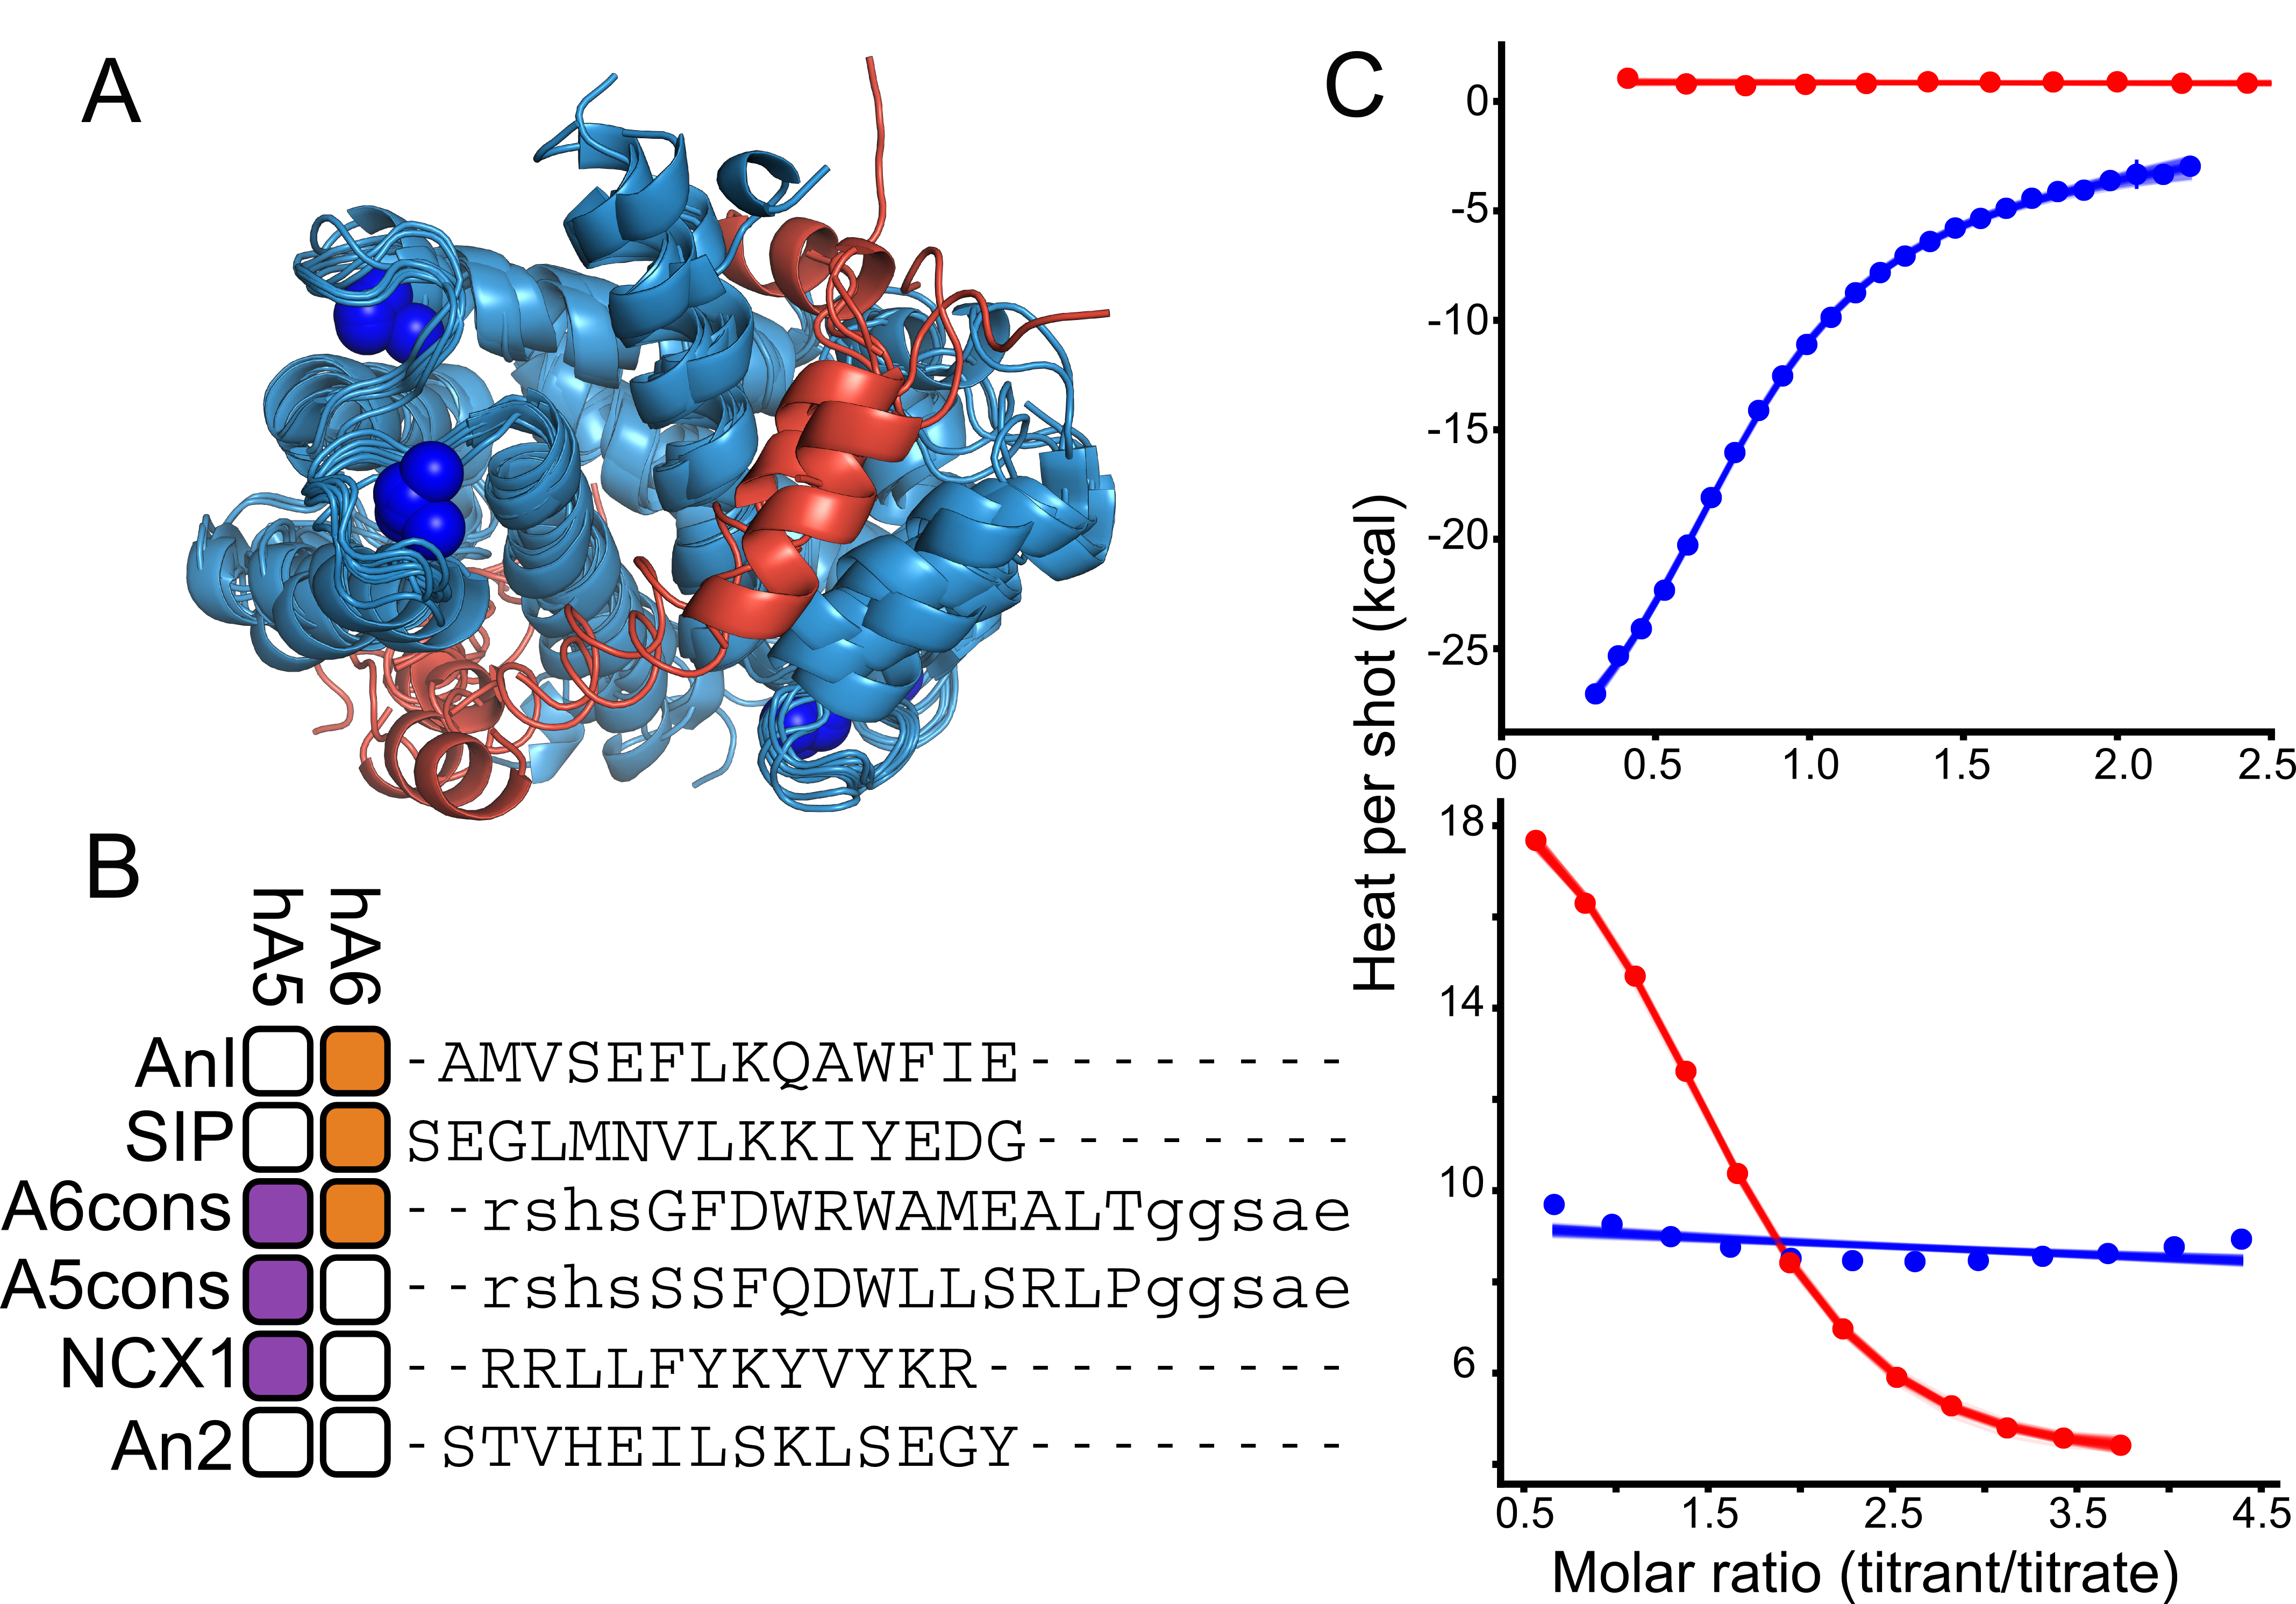
\includegraphics{ch5-fig1.png} 
\caption[Human S100A5 and S100A6 exhibit peptide binding specificity]{Human S100A5 and S100A6 exhibit peptide binding specificity. A) Published structures of S100 family members bound to both $Ca^{2+}$
and peptide targets at the canonical hydrophobic interface (PDB: 3IQQ, 1QLS, 3RM1, 2KRF, 4ETO, 2KBM, 1MWN, 3ZWH). Structures are aligned
to the $Ca^{2+}$--bound structure of human S100A5 (2KAY). Peptides
are shown in red. Blue spheres are $Ca^{2+}$ ions. B) Binding specificity
of hA5 and hA6. Boxes indicate whether the peptide binds to hA5 (purple)
and/or hA6 (orange). If peptide does not bind by ITC ($K_{D}$ $>$100 $\mu M$),
the box is white. Peptide names are indicated on the left. Peptide
sequences, aligned using MUSCLE \citep{edgar_muscle:_2004}, are shown
on the right. Solubilizing flanks, which contribute minimally to binding
(Table 3 in supplement), are shown in lowercase letters. Annexin 1 (An1) and Annexin
2 (An2) binding measurements are from a published study \citep{streicher_annexin_2009}.
C) ITC heats for the titration of NCX1 (blue) and SIP (red) peptides
onto hA5 (top) and hA6 (bottom). Points are integrated heats extracted
from each shot. Lines are 100 different fit solutions drawn from the
fit posterior probability distributions. For the hA5/NCX1
and hA6/SIP curves, we used a single--site binding model. For hA5/SIP
and hA6/NCX1, we used a blank dilution model. Thermodynamic parameters
for these fits are in Table 4--7 in supplement.\label{samplefigure}}	
\end{figure}

\section{Results}

\subsection{Human S100A5 and S100A6 interact with diverse peptides at the same
binding site}

We first systematically compared the binding specificity of human
S100A5 (hA5) relative to human S100A6 (hA6) for a collection of six
peptides (Fig 14B). Peptide targets have been reported for both hA5
and hA6 \citep{lee_structure_2008,leclerc_binding_2009,slomnicki_s100a6_2009,streicher_annexin_2009,van_dieck_modulation_2009,liriano_structure_2012,cho_pentamidine_2016},
but only two targets have been directly compared between paralogs.
Using Isothermal Titration Calorimetry (ITC), Streicher and colleagues
found that a peptide fragment of Annexin 1 bound to hA6 but not hA5,
and a peptide fragment of Annexin 2 bound to neither \citep{streicher_annexin_2009}
(Fig 14B). To better quantify the relative specificity of these proteins,
we used ITC to measure the binding of two additional peptides to recombinant
hA5 and hA6. The first was a peptide from Siah--interacting protein
(SIP) previously reported to bind to hA6 \citep{lee_structure_2008}.
We found that this peptide bound to hA6 with a $K_{D}$ of $20\ \mu M$,
but did not bind hA5 (Fig 14B, C). The second was a 12 amino acid fragment
of the protein NCX1 that was reported to bind to hA5 \citep{liriano_structure_2012}.
We found that this peptide bound with to hA5 with a $K_{D}$ of $20\ \mu M$,
but did not bind hA6 (Fig 14B, C). 

To further characterize the specificity of the interface, we used
phage display to identify two additional peptides that bound to each
protein. We panned a commercial library of random 12--mer peptides
fused to M13 phage with either hA5 or hA6. Phage enrichment was strictly
dependent on $Ca^{2+}$ (Fig 32 in supplement). Three sequential rounds of binding
and amplification with either hA5 or hA6 led to enrichment of the
``A5cons'' and ``A6cons'' peptides (Fig 15B, Fig 32 in supplement). We then used
ITC to measure binding of these peptides to hA5 and hA6. To ensure
solubility, we added polar N and C--terminal flanks before characterizing
binding. A5cons bound to both hA5 and hA6 (Fig 14C). In contrast, A6cons,
bound hA6 but not hA5 (Fig 14C). To verify that binding was driven
by the central region, we re--measured binding in the presence and
absence of different versions of the flanks (Table 3 in supplement). 

The peptides that bind to hA5 and hA6 are diverse in sequence, hydrophobicity,
and charge (Fig 14B). One explanation for this diversity could be that
the peptides bind at different interfaces on the protein. To test
for this possibility, we used NMR to identify residues whose chemical
environment changed on binding of peptide. We first verified the published
assignments for hA5 using a 3D NOESY--TROSY experiment \citep{bertini_solution_2009}.
We then collected $^{1}H-^{15}N$ TROSY--HSQC NMR spectra of $Ca^{2+}$--bound
protein in the presence of either the A5cons or A6cons peptide. By
comparing the bound and unbound spectra, we could identify peaks whose
location shifted dramatically or that broadened due to exchange. In
addition to our own work, we also included previously reported experiments
probing the hA5/NCX1 peptide interaction in the analysis \citep{liriano_structure_2012}.
For all three peptides, we observed a consistent pattern of perturbations
in helices 3 and 4 and, to a lesser extent, helix 1 upon peptide binding
(Fig 15A--C). These results suggest that all three peptides bind at
the canonical interface. In addition to this spectroscopic evidence,
binding of all of these peptides was strictly dependent on the presence
of $Ca^{2+}$ (Fig 15D--F)---consistent with binding at the interface
exposed on $Ca^{2+}$ binding \citep{bertini_solution_2009}.

\begin{figure}
\centering
	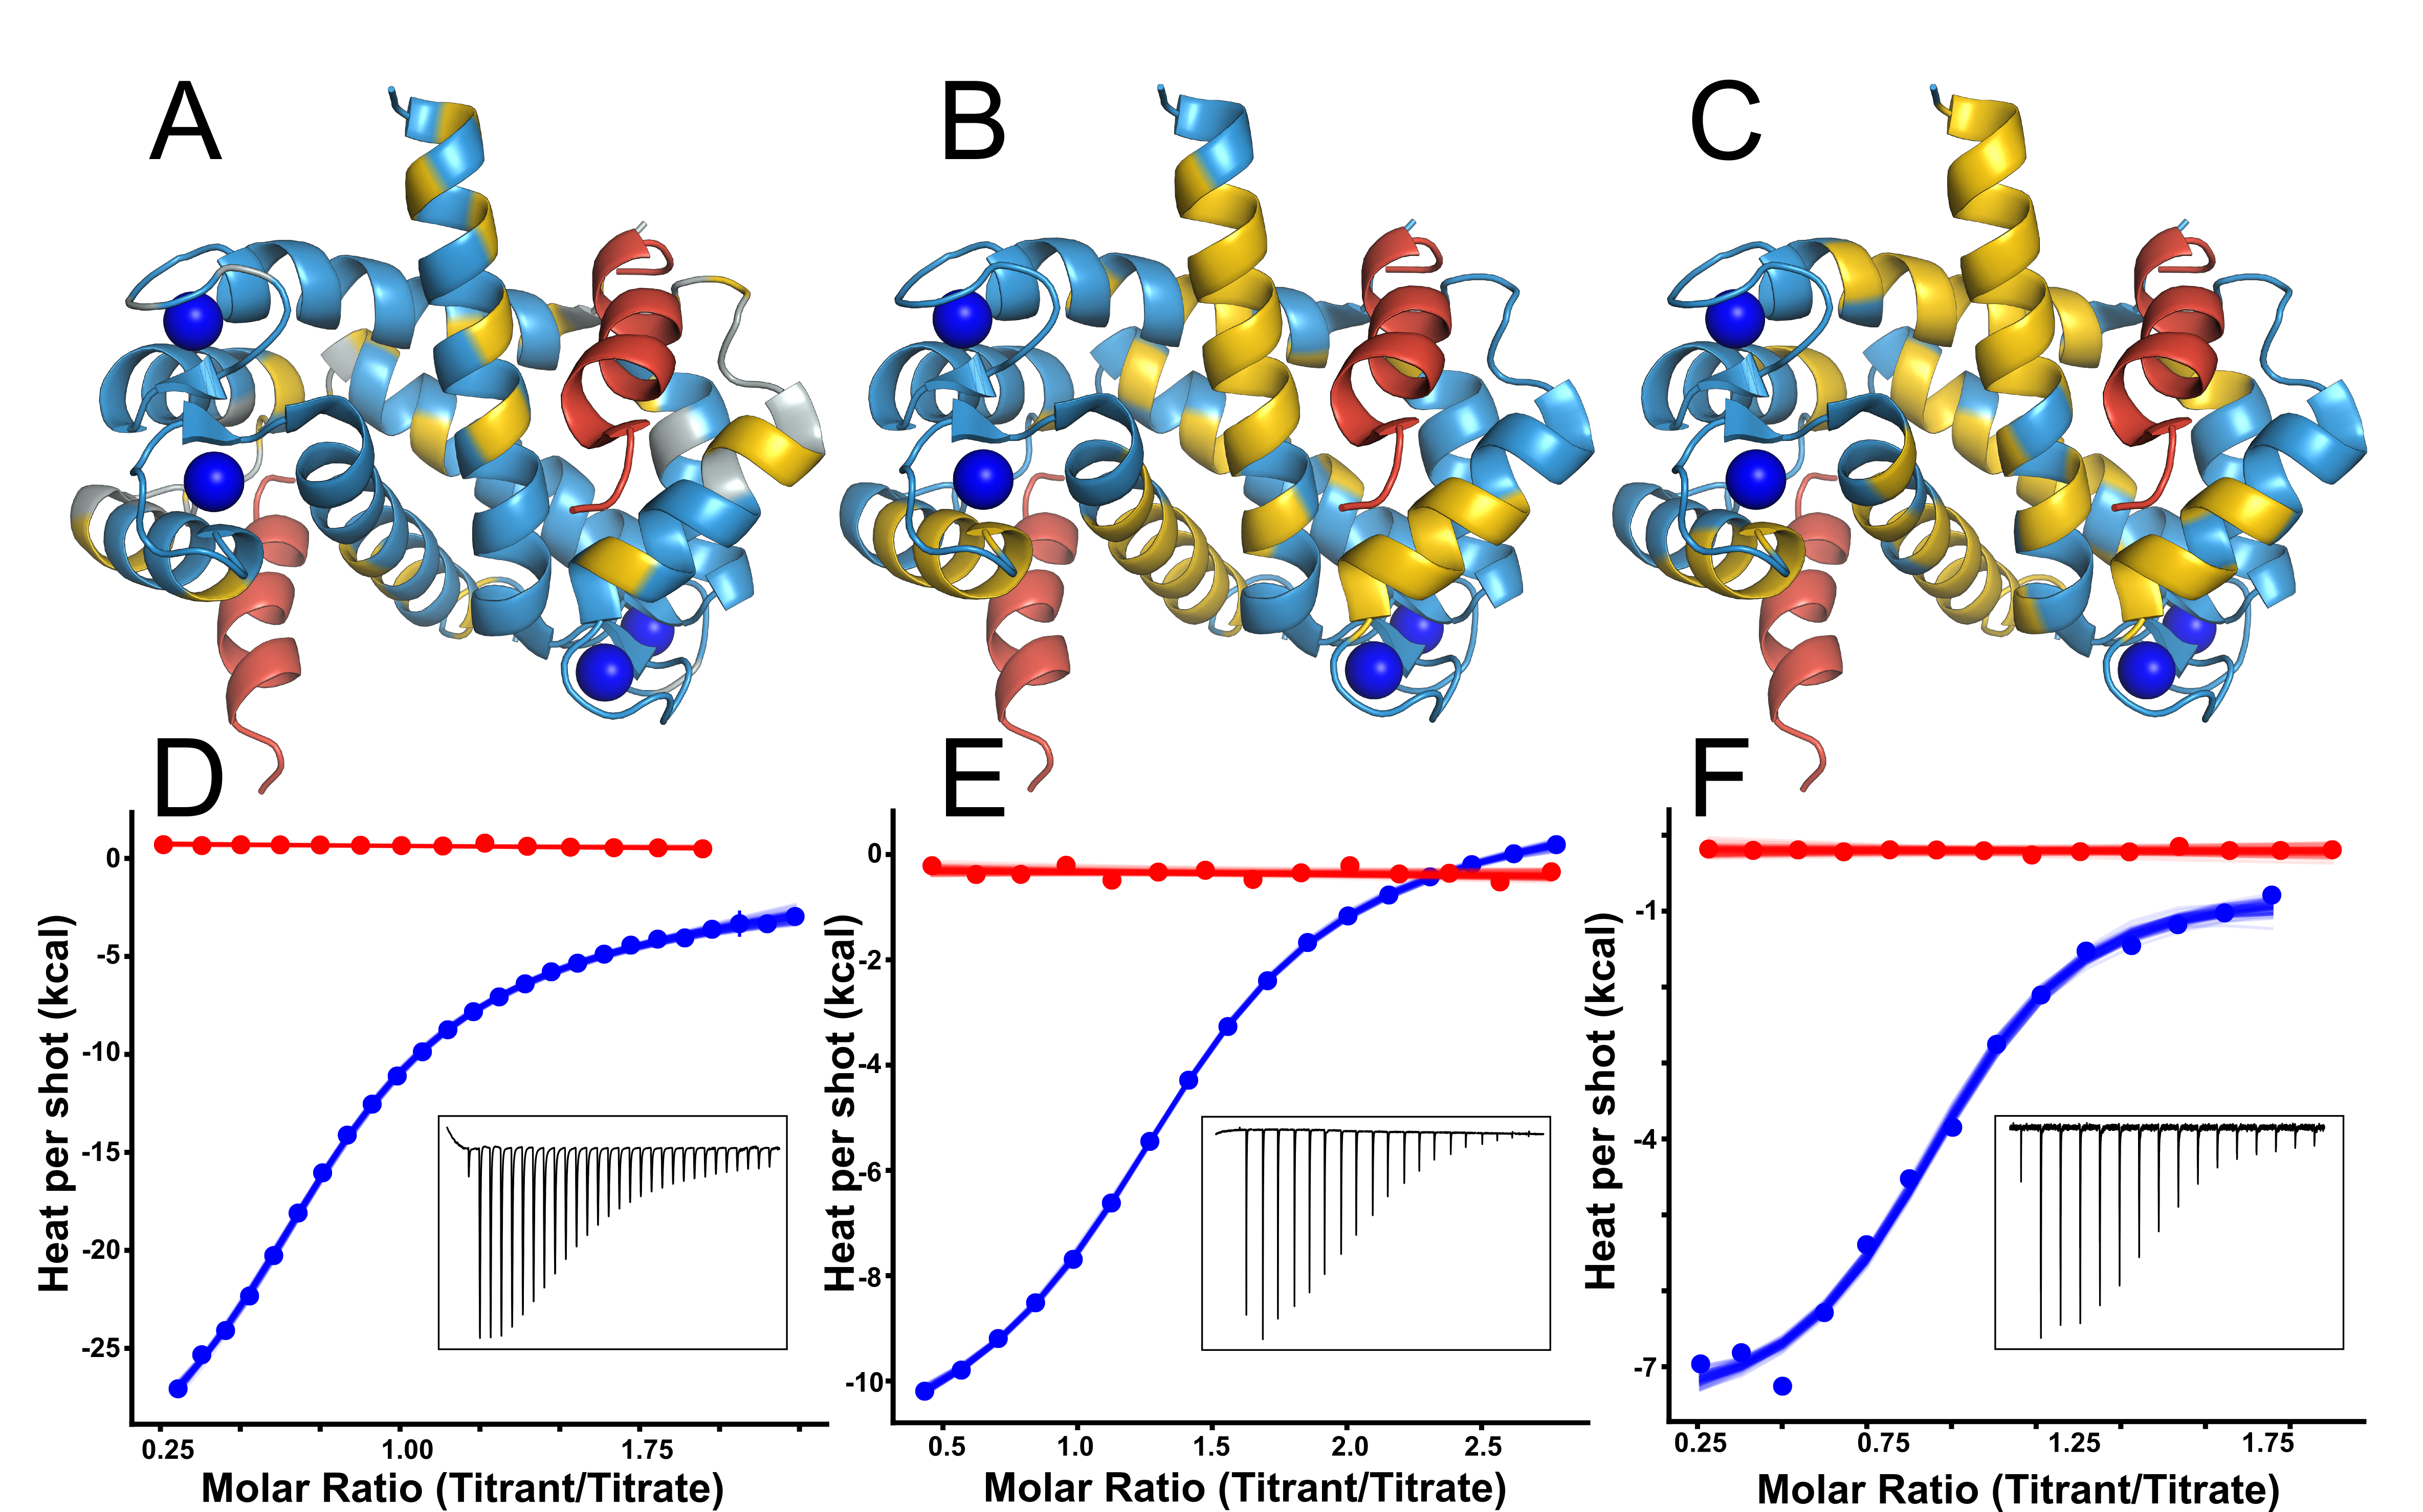
\includegraphics{ch5-fig2.png} 
\caption[Diverse peptides bind at the human S100A5 peptide interface]{Diverse peptides bind at the human S100A5 peptide interface.Structures show NMR data mapped onto the structure of $Ca^{2+}$--bound
hA5 (2KAY \citep{bertini_solution_2009}). To indicate the expected
peptide binding location, we aligned a structure of hA6 in complex
with the SIP peptide (2JTT \citep{lee_structure_2008}) to the hA5
structure, and then displayed the SIP peptide in red. Panels A--C show
binding for NCX1, A5cons, and A6cons respectively. In panel A, yellow
residues are those noted as responsive to NCX1 binding in \citep{liriano_structure_2012}.
In panels B and C, yellow residues are those whose $^{1}H$--$^{15}N$
TROSY--HSQC peaks could not be identified in the peptide--bound spectrum
because the peaks either shifted or broadened. Panels D--E show ITC
data for binding of the peptides above in the presence of 2 mM $Ca^{2+}$
(blue) or 2 mM EDTA (red). Points are integrated heats extracted from
each shot. Lines are 100 different fit solutions drawn from the fit
posterior probability distributions. For the $Ca^{2+}$ curves,
we used a single--site binding model. For the EDTA curves, we used
a blank dilution model. Insets show raw ITC power traces for the $Ca^{2+}$
binding curves. Thermodynamic parameters for these fits are in Table
4--7 in supplement.\label{samplefigure}}	
\end{figure}

\subsection{The S100A5 and S100A6 clades exhibit conserved binding specificity}

Although hA5 and hA6 bind to diverse peptide targets at the same interface,
they exhibit distinct specificity relative to one another (Fig 14B).
The particular peptides that bind or not could be random if specificity
fluctuates over evolutionary time. In contrast, if specificity at
the interface is strongly constrained, we would expect conserved specificity
between paralogs. We therefore set out to study the evolution of the
differences in peptide binding between the human proteins. 

\begin{figure}
\centering
	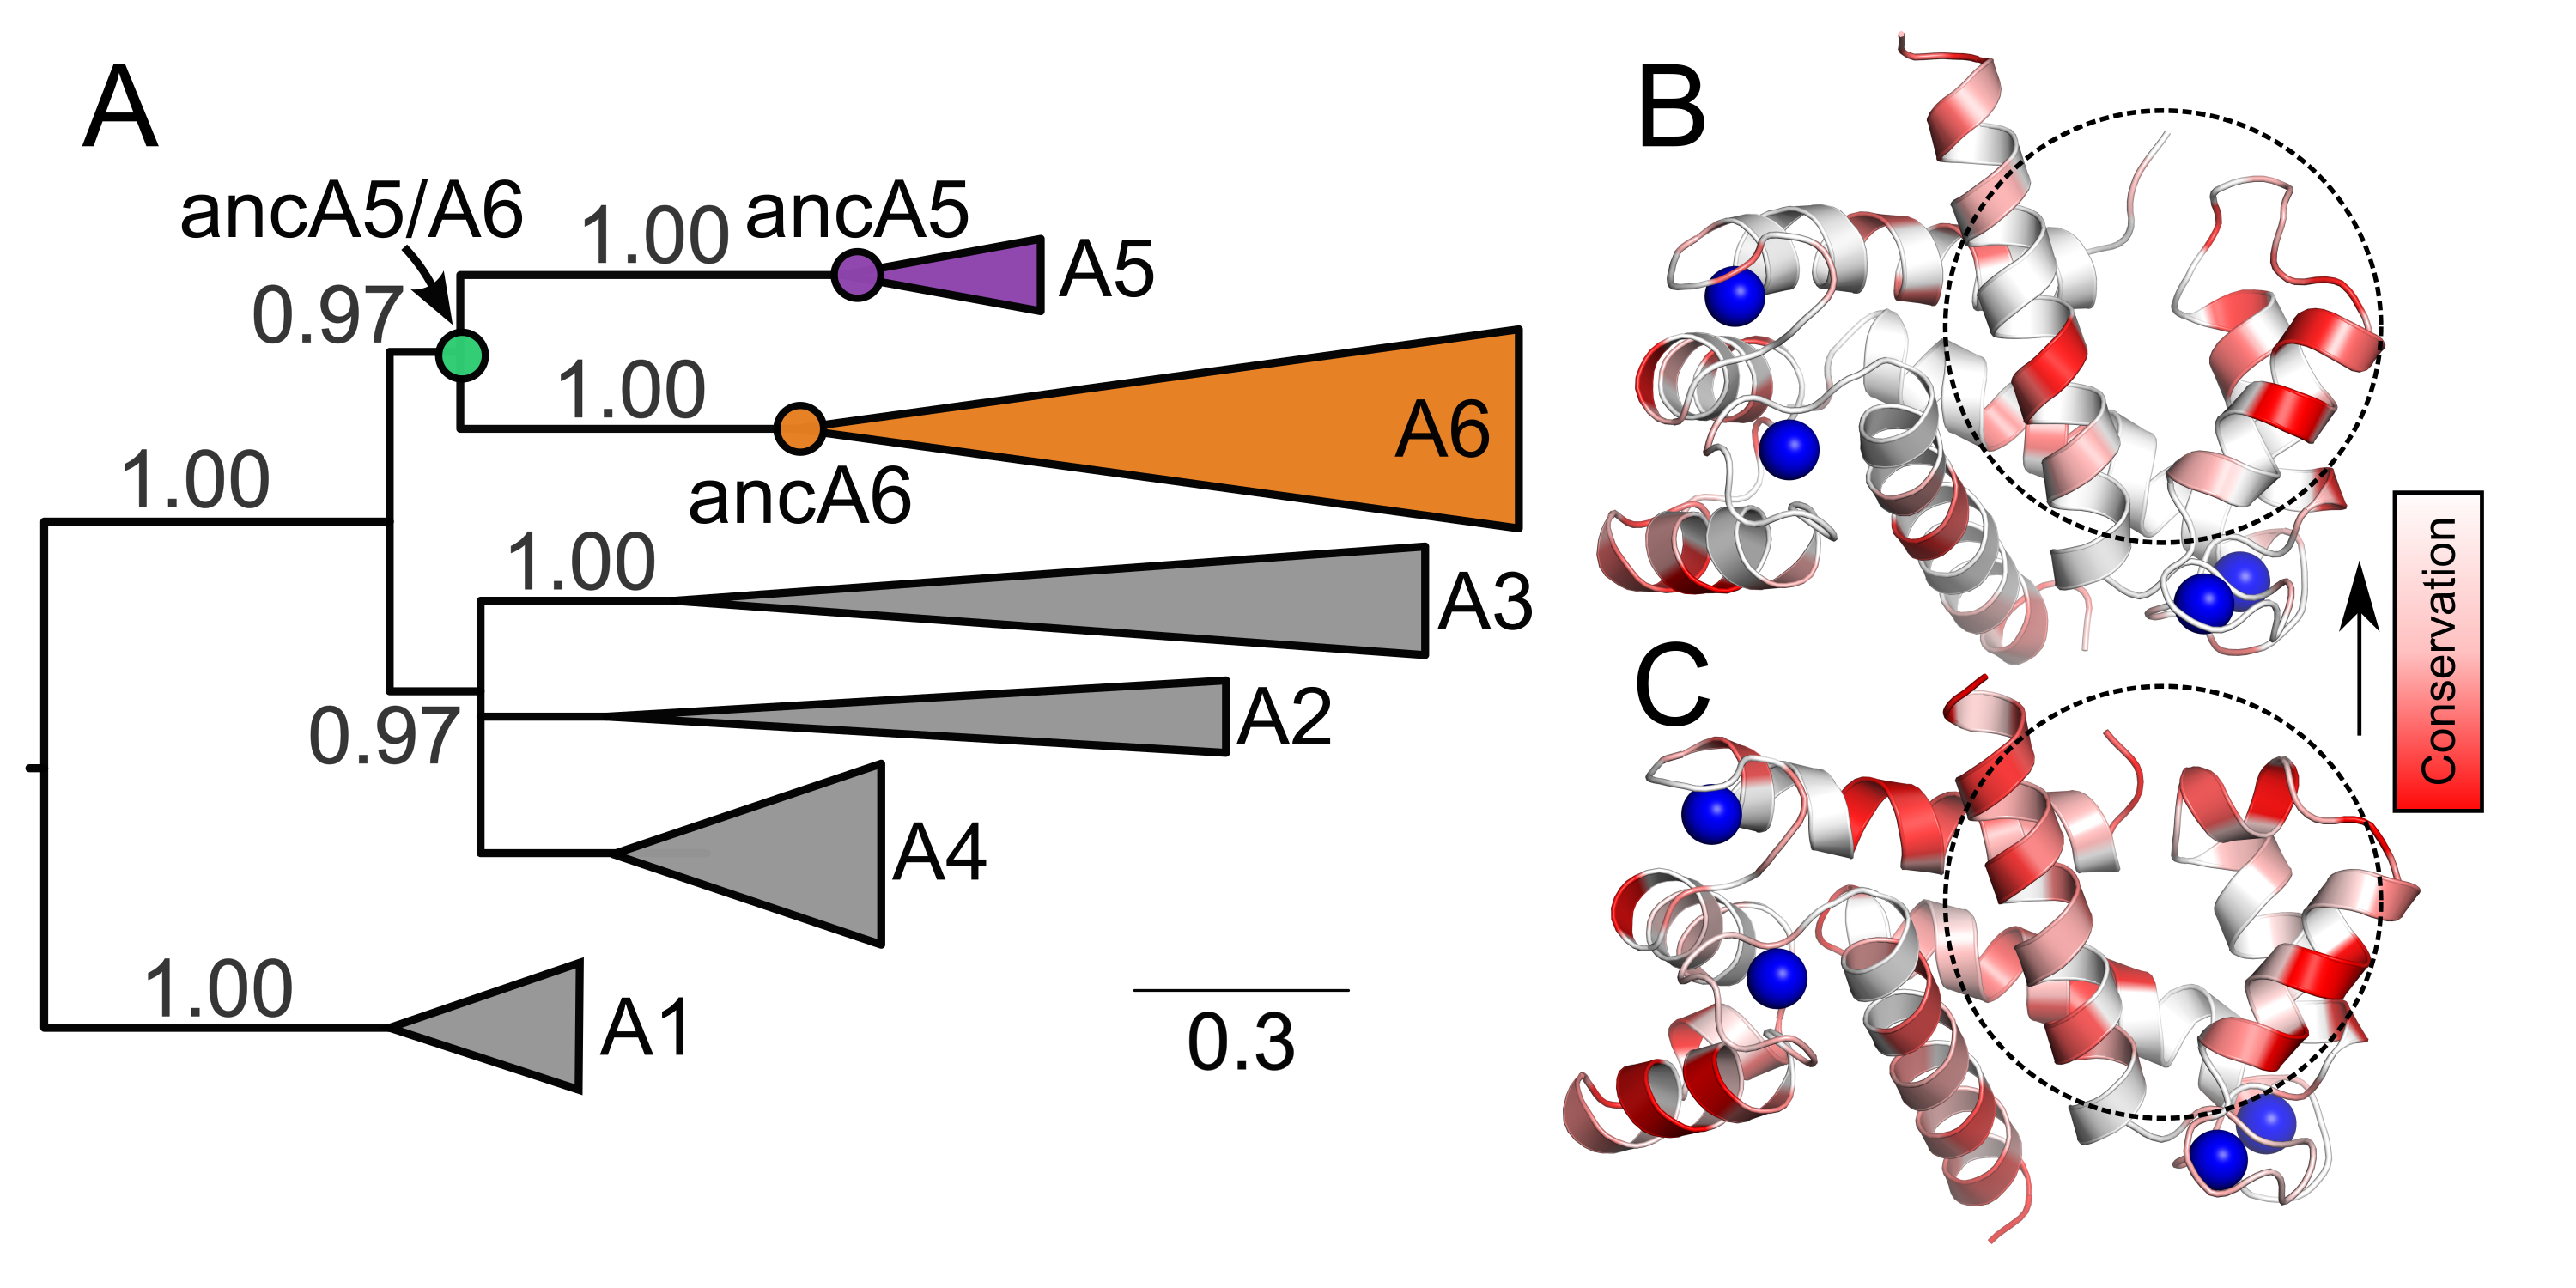
\includegraphics{ch5-fig3.png} 
\caption[S100A5 and S100A6 arose by gene duplication]{S100A5 and S100A6 arose by gene duplication in the
amniote ancestor. A) Maximum likelihood phylogeny for S100A5, S100A6
and their close homologs. Wedges denote collections of paralogs (S100A1,
S100A2, S100A3, S100A4, S100A5, or S100A6). Wedge height corresponds
to the number of sequences and wedge length to the longest branch
in that clade. SH supports, estimated using an approximate likelihood
ratio test \citep{guindon_new_2010}, are shown above the branches.
Scale bar shows branch length in substitutions per site. Reconstructed
ancestors are denoted with circles. All proteins, with the exception
of those in the A1 clade, are taken from amniotes. A1 contains S100
proteins from bony vertebrates and was used as an out--group to root
the tree. Panels B and C show relative conservation of residues across
amniote paralogs mapped onto the structures of hA5 (2KAY, \citep{bertini_solution_2009})
and hA6 (1K96, \citep{otterbein_crystal_2002}). Colors denote conservation
from $<20\ \%$ (dark red) to $100\ \%$ white. Sequences were taken
from the alignment used to generate the phylogeny in panel A. Dashed
circles denote the peptide binding surface for one of the two chains.
Blue spheres show the location of bound $Ca^{2+}$ in the structures.\label{samplefigure}}	
\end{figure}

We first constructed a maximum--likelihood phylogeny of the clade containing
S100A2, S100A3, S100A4, S100A5, and S100A6 (Fig 16A). We built the
tree using the EX/EHO+$\Gamma_{8}$ evolutionary model \citep{le_accounting_2010},
which uses different evolutionary models for sites in different structural
classes. As expected from previous phylogenetic and syntenic analyses
\citep{zimmer_evolution_2013,wheeler_multiple_2016}, S100A5 and S100A6
were paralogs that arose by gene duplication in the amniote ancestor,
with S100A2, S100A3, and S100A4 forming a closely--related out group
(Fig 16A). To set our expectation for conservation of specificity,
we then calculated the conservation of residues at the binding site
across S100A5 and S100A6 homologs. Fig 16B and C show the relative
conservation of residues on hA5 (Fig 16B) and hA6 (Fig 16C). Taken as
a whole, the peptide binding region does not exhibit higher conservation
than other regions in the protein. We therefore predicted substantial
variability in the peptide binding specificity across S100A5 and S100A6
orthologs. 

To test the prediction that specificity has fluctuated over time,
we expressed and purified S100A5 and S100A6 orthologs from human,
mouse (\textit{Mus musculus}), tasmanian devil (\textit{Sarcophilus harrisii}),
American alligator (\textit{Alligator mississippiensis}), and chicken
(\textit{Gallus gallus}). We then characterized the peptide binding
specificity of these S100A5 and S100A6 orthologs against four peptides:
A5cons, A6cons, SIP, and NCX1 (Fig 17A). We selected these peptides
because there is direct evidence that these peptides bind at the canonical
binding interface (Fig 15, as well as \citep{lee_structure_2008,liriano_structure_2012}).
Surprisingly, we found that the S100A5 and S100A6 clades exhibited
broadly similar, ortholog--specific binding specificity (Fig 17A). All
S100A5 orthologs bound NCX1, A5cons, and A6cons, but not SIP. In contrast,
all S100A6 orthologs bound SIP and A6cons, but not A5cons. The only
labile character is NCX1 binding to S100A6. The sauropsid and marsupial
S100A6 orthologs bound NCX1, but not the eutherian mammal representatives.
We also characterized binding of these peptides to human S100A4 as
an outgroup. Binding for this protein was intermediate between the
S100A5 and S100A6 clades: it bound A5cons and A6cons, but not SIP
or NCX1. Thermodynamic parameters for these binding experiments are
given in Table 4--7 in supplement. Representative ITC traces for each protein are
shown in Fig 33 in supplement. 

\begin{figure}
\centering
	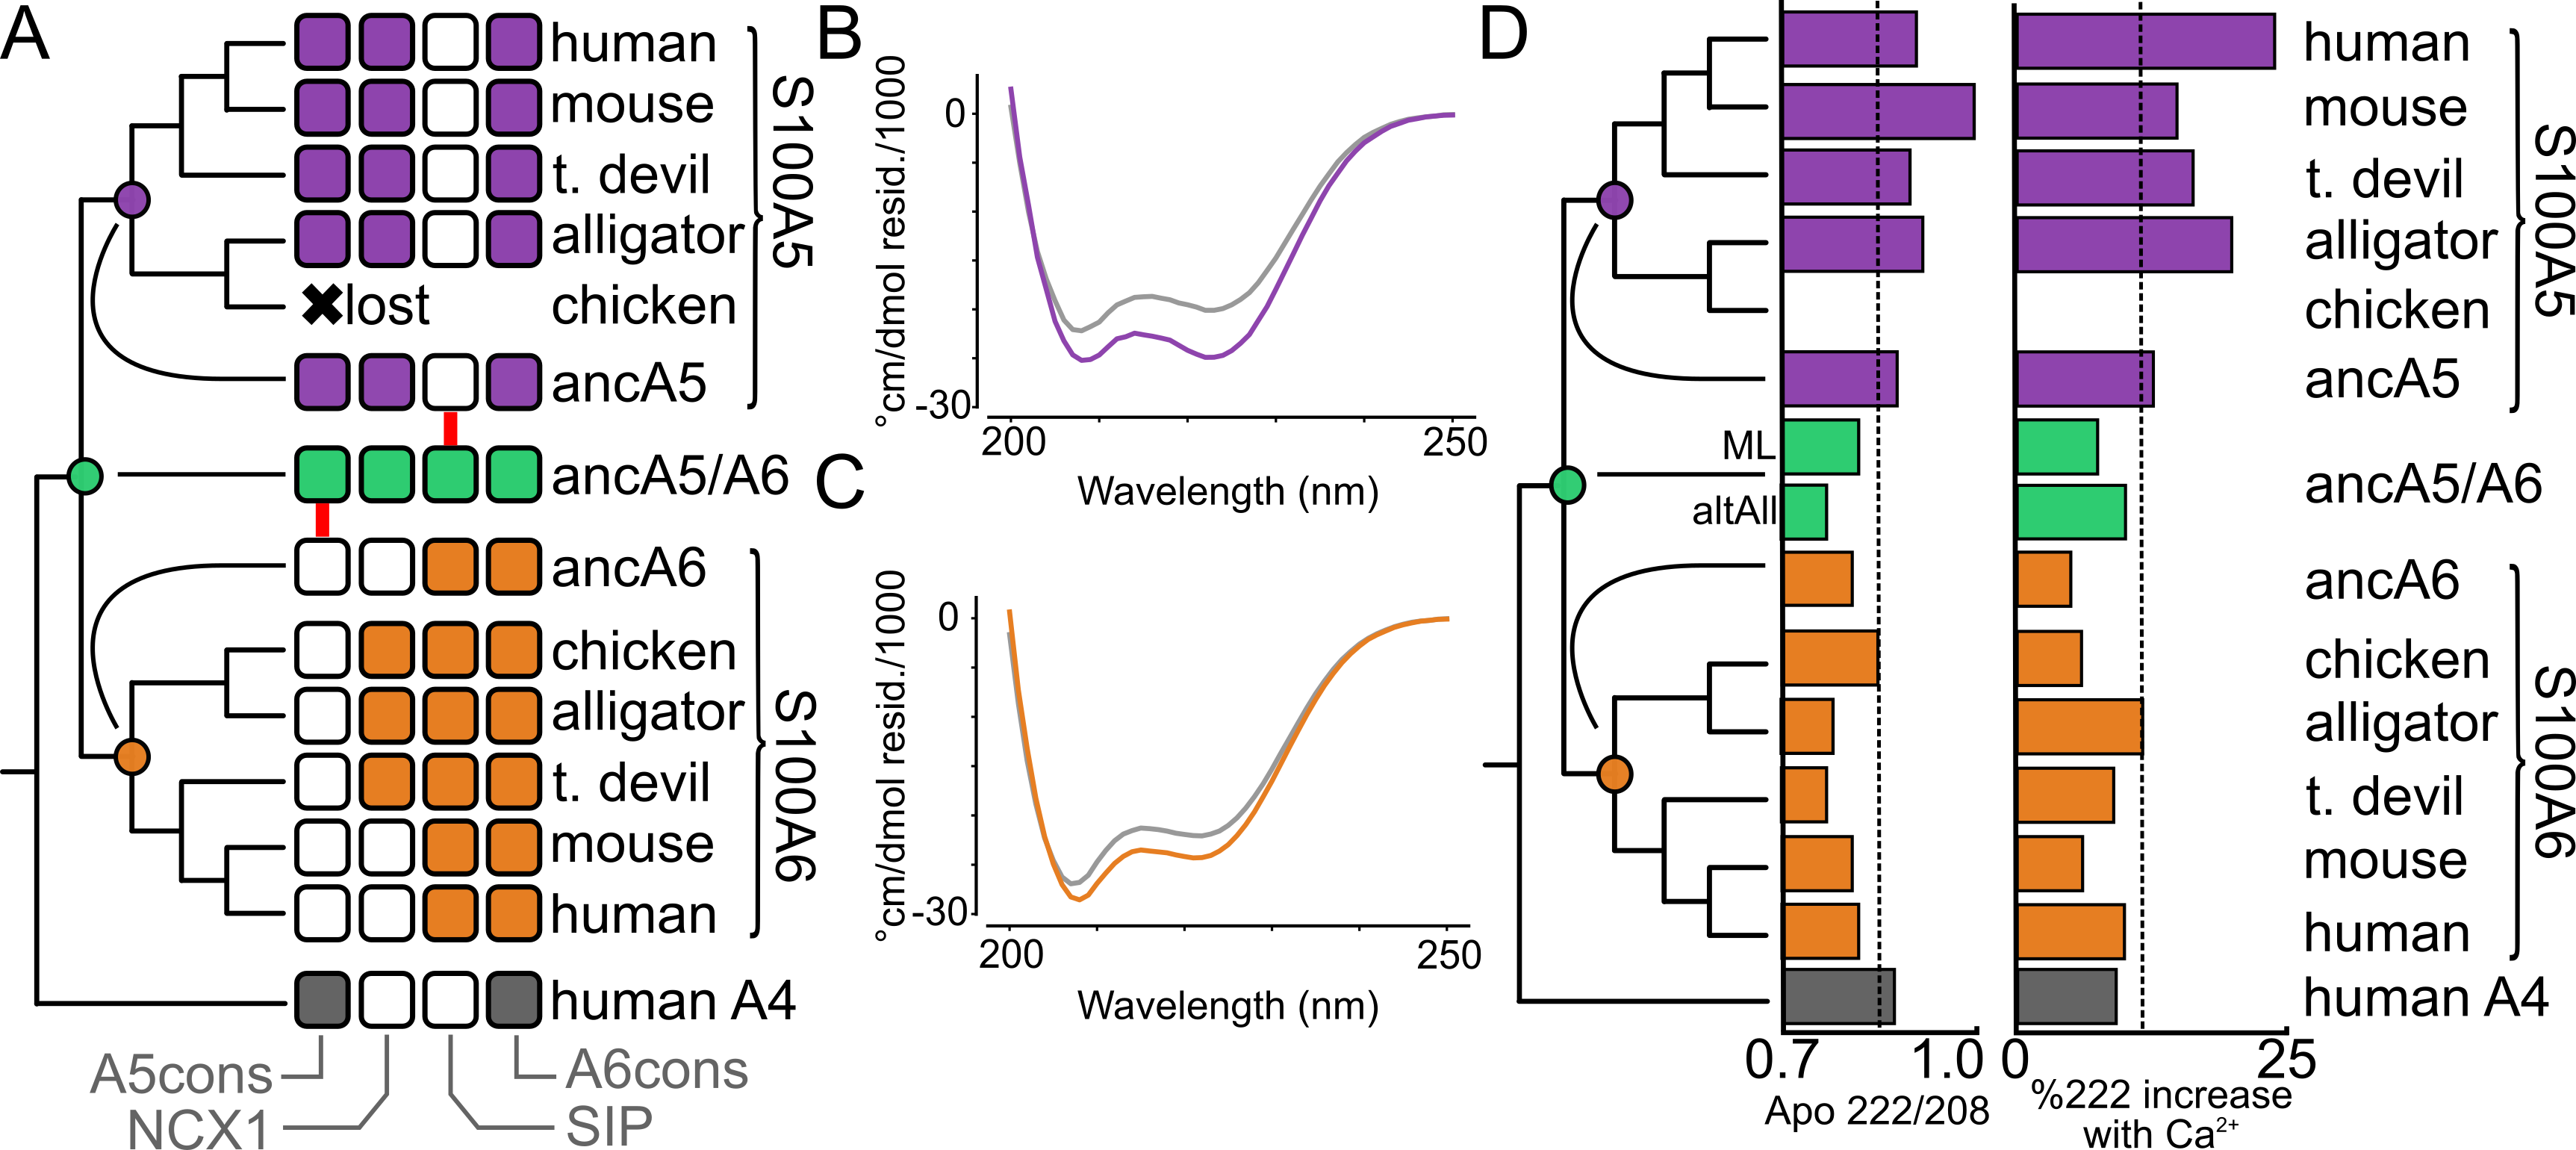
\includegraphics{ch5-fig4.png} 
\caption[S100A5 and S100A6 paralogs exhibit conserved properties]{S100A5 and S100A6 paralogs exhibit conserved properties.A) Peptide binding specificity mapped onto the phylogenetic tree as
a collection of binary characters. Each square denotes binding of
a specific peptide to an ortholog sampled from the species indicated
at right. Squares are filled if binding was observed by ITC. Ancestors
are shown in the middle, with red arrows indicating changes that occurred
after duplication that were then conserved across orthologs. The results
for ancA5/A6 were identical for both the ML and ``altAll'' ancestors.
Full thermodynamic parameters are in Table 4--7 in supplement. B) Far--UV spectra
for apo (gray) and $Ca^{2+}$--bound (purple) hA5. C) Far--UV spectra
for apo (gray) and $Ca^{2+}$--bound (orange) hA6. D) Spectroscopic
properties mapped onto the phylogeny. The left column shows the ratio
of absorbance at 222 nm/208 nm for the apo protein. The right column
shows the percentage increase in signal at 222 nm upon addition of
$Ca^{2+}$. Dashed lines show the mean values across all experiments.
Raw spectra are given in Fig 34 in supplement.\label{samplefigure}}	
\end{figure}

The strong conservation of peptide binding suggested that other features---such
as structural features---might be conserved between paralogs as well.
To test for this, we characterized the secondary structure and response
to $Ca^{2+}$ for all proteins using far--UV circular dichroism (CD)
spectroscopy. A $Ca^{2+}$--driven change in $\alpha$--helical secondary
structure is a conserved feature of S100 proteins \citep{wheeler_multiple_2016,marenholz_s100_2004}.
We asked whether this behavior was conserved across orthologs, which
would indicate similar structural properties. As with peptide binding,
we found that the CD spectrum and response to $Ca^{2+}$ were diagnostic
within each clade (Fig 17B--D, Fig 34 in supplement). S100A5 orthologs exhibited deep
minima at 208 and 222 nm, corresponding to a largely $\alpha$--helical
secondary structure (Fig 17B,D). This signal increased upon addition
of saturating $Ca^{2+}$, consistent with the ordering of the C--terminus
of the human protein reported by NMR \citep{bertini_solution_2009}.
In contrast, all S100A6 orthologs exhibited a deeper minimum at 208
nm, likely corresponding to a mixture of $\alpha$--helical and random
coil secondary structure. The secondary structure of these proteins
changed comparatively little on addition of $Ca^{2+}$ (Fig 17C,D). 

\subsection{Specificity evolved from an apparently promiscuous ancestor}

Surprisingly, despite the diversity of peptides that bind to each
paralog, peptide binding specificity is conserved across across paralogs.
We next asked whether these proteins exhibited comparable evolutionary
patterns to those observed in high--specificity proteins, such as the
partitioning of ancestral binding partners along duplicate lineages
\citep{eick_evolution_2012,hudson_distal_2015,clifton_ancestral_2016}.
Using our phylogeny, we used ancestral sequence reconstruction (ASR)
to reconstruct the last common ancestors of S100A5 orthologs (ancA5)
and S100A6 orthologs (ancA6) \citep{yang_new_1995}. These proteins
were well reconstructed, having mean posterior probabilities of 0.93
and 0.96, respectively. Their sequences are given in Table 8 in supplement. We
expressed and purified both of these proteins. We found that they
shared similar secondary structures and $Ca^{2+}$--binding responses
with their descendants by far--UV CD (Fig 17C). We then measured binding
to the suite of four peptides described above using ITC. These ancestors
gave the pattern we would expect given the binding specificities of
the derived proteins (Fig 17D). AncA5 is indistinguishable from a modern
S100A5 ortholog, binding A5cons, A6cons, and NCX1, but not SIP (Fig
4D). AncA6 also behaves as expected, binding A6cons and SIP, but not
A5cons. It does not bind NCX1, consistent with this character being
labile in the S100A6 lineage (Fig 17D). 

We next characterized the last common ancestor of S100A5 and S100A6 (ancA5/A6).
This reconstruction had a mean posterior probability of 0.83 (Table
S6). AncA5/A6 has a secondary structure content identical to ancA6
and the S100A6 descendants. It also responds to $Ca^{2+}$ in a similar
fashion (Fig 17C, Fig 33 in supplement). Unlike any modern protein, however, ancA5/A6
binds to all four peptides (Fig 18). To verify that this result was
not an artifact of the reconstruction, we also made an ``AltAll''
ancestor of ancA5/A6 in which we swapped all ambiguous sites in the
maximum--likelihood ancestor with their next most likely alternative
\citep{eick_robustness_2017} (Table 8 in supplement, methods). This protein is
quite different than ancA5/A6---differing at 21 of 93 sites---but the
binding profile for the four peptides was identical to the maximum--likelihood
ancestor. Thermodynamic parameters for these binding experiments are
given in Table 4--7 in supplement. 

\subsection{Binding specificity can be changed with a single mutation}

Our work revealed that S100A5 and S100A6, despite having low overall
specificity, display the same basic evolutionary patterns as high--specificity
proteins \citep{eick_evolution_2012,clifton_ancestral_2016,alhindi_protein_2017}:
they exhibit conserved partners across modern orthologs and display
a pattern of subfunctionalization from a less specific ancestor. While
suggestive, this does not establish that there is selection to maintain
specificity. Another possibility is that switching specificity is
intrinsically difficult, and that the pattern we observe reflects
this difficulty rather than selective pressure to maintain a particular
specificity profile. 

To distinguish these possibilities, we attempted to shift the binding
specificity of hA5 by introducing mutations at the binding interface.
We selected five historical substitutions that occurred along the
branch between ancA5/A6 and ancA5: e2A, i44L, k54D, a78M, m83A (with
the ancestral amino acid in lowercase and modern amino acid in uppercase).
We chose these substitutions using three criteria: 1) the ancestral
amino acid was conserved in S100A6 orthologs, 2) the derived amino
acid was conserved in S100A5 orthologs, 3) and the mutations were
located at the peptide binding interface. Fig 18A shows the positions
of candidate substitutions mapped onto the structure of hA5 \citep{bertini_solution_2009}.

\begin{figure}
\centering
	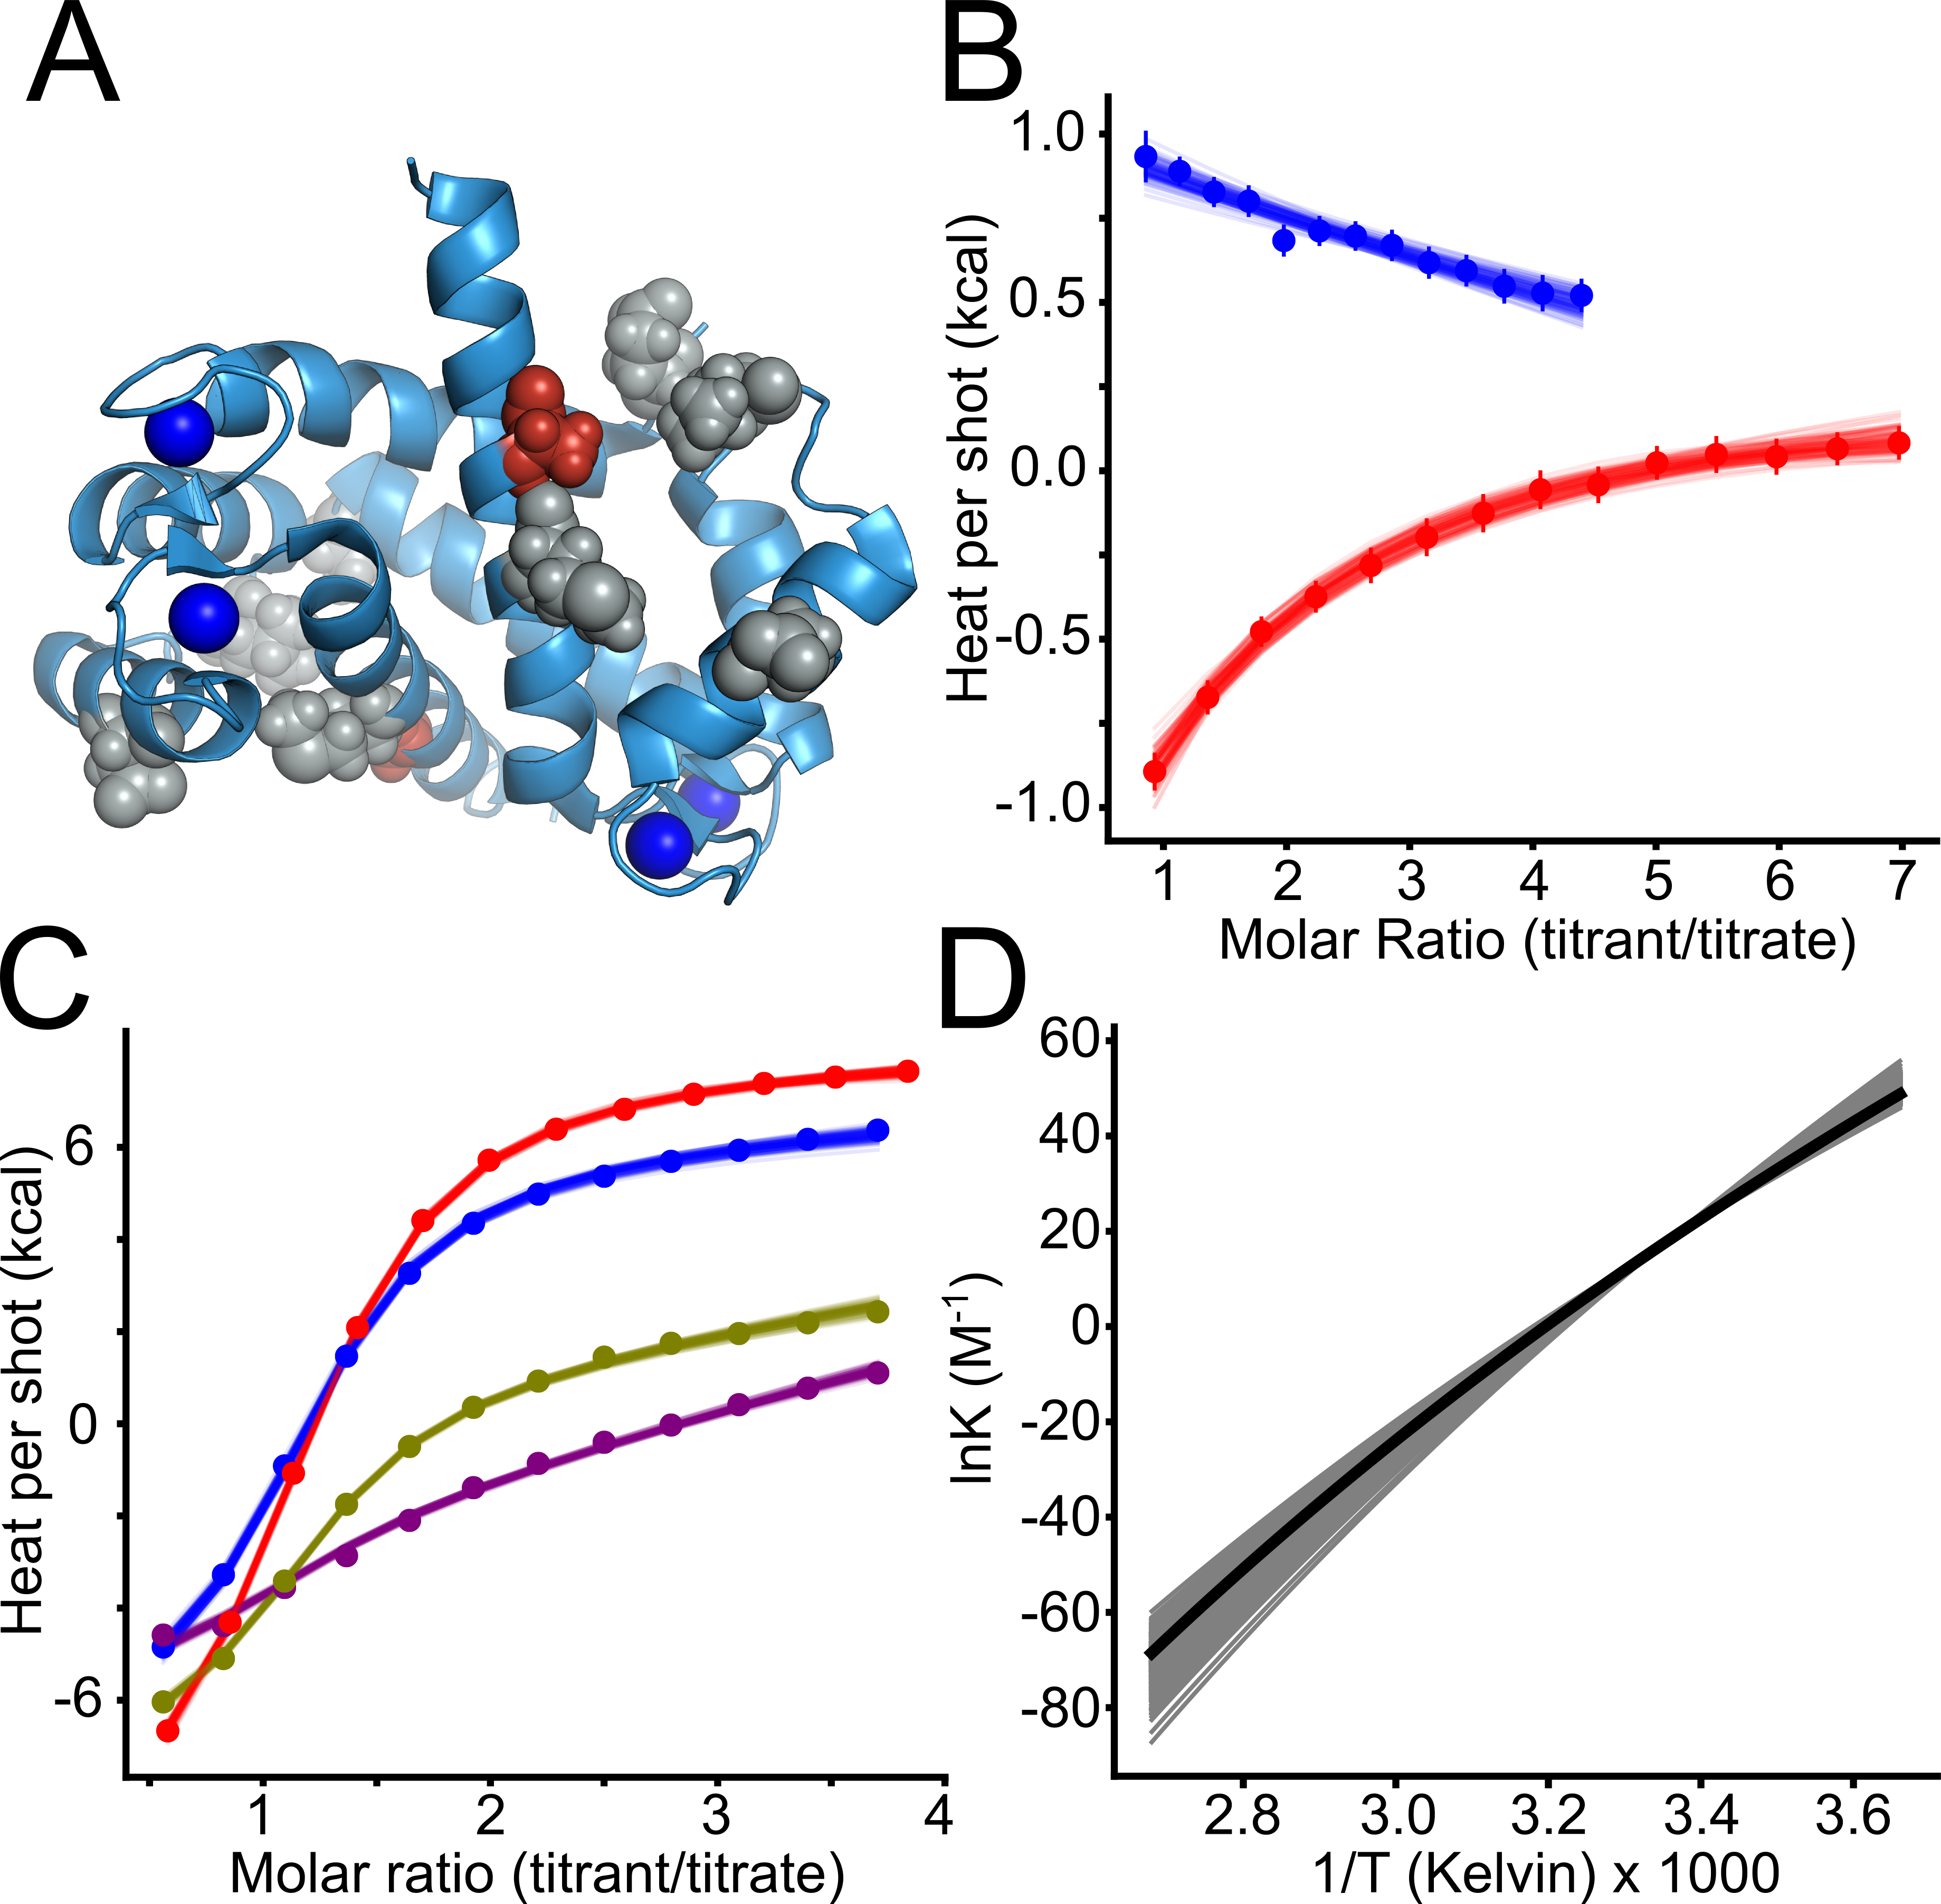
\includegraphics{ch5-fig5.png} 
\caption[Small changes are sufficient to alter binding specificity]{Small changes are sufficient to alter binding specificity
at the interface. A) $Ca^{2+}$--bound structure of human S100A5 (2KAY)
\citep{bertini_solution_2009} with ancestral reversions marked in
gray (no effect on SIP binding) and red (A83m---allows SIP binding).
Blue spheres are $Ca^{2+}$ ions. B) ITC traces showing titration
of SIP onto hA5 A83m (red) versus wildtype hA5 (blue). ITC experiments
were performed at $25{^\circ}C$ in 25 mM TES, 100 mM NaCl, 2 mM $CaCl_{2}$,
1mM TCEP, pH 7.4. Points are integrated heats extracted from each
shot. For each experiment, we sampled fit parameters using Bayesian
Markov Chain Monte Carlo as implemented in pytc. For the A83m curve,
we used a single--site binding model. For the wt curve, we used a blank
dilution model, where the linear slope is indicative of peptide dilution
without binding. Lines are 100 different solutions drawn from the
Bayesian posterior probability distributions.\textbf{ }C) ITC traces
from experiments done at multiple temperatures: $10{^\circ}C$ (purple),
$15{^\circ}C$ (green), $20{^\circ}C$ (blue), and $25{^\circ}C$
(red). Experiments were performed in 25mM TES, 100mM NaCl, 2mM $CaCl_{2}$,
1mM TCEP, pH 7.4. Dots are integrated heats with uncertainty calculate
using NITPIC \citep{keller_high-precision_2012}. There is a clear
temperature dependence of the binding enthalpy. A global Van't Hoff
model was fit to the data using the Bayesian MCMC fitter in pytc.
We were unable to fit the model without inclusion of a $\Delta C_{p}^{\circ}$
parameter ($-0.40\text{\ensuremath{\le}}-0.36\text{\ensuremath{\le}}-0.32kcal\cdot mol^{-1}\cdot K^{-1}$),
suggesting that there is a change in heat capacity as a function of
temperature, which is indicative of a hydrophobically--driven interaction.
Lines are 100 curves drawn from the posterior distribution of the
fits. Table 9 in supplement. D) Van't Hoff plot of temperature dependence data.
Thick black line shows Maximum Likelihood curve, gray lines are 500
curves drawn from the posterior distribution of the Bayesian fit.
There is slight, but detectable curvature in the plot, consistent
with the small $\Delta C_{p}^{\circ}$ parameter obtained from global
model.\label{samplefigure}}	
\end{figure}

We reversed each of these sites individually to the ancestral state
in hA5. We then measured binding of two clade--specific peptides, SIP
and A5cons, to each mutant using ITC (Table 9 in supplement). We found that reverting
a single substitution (A83m) to its ancestral state in hA5 enabled
it to bind the SIP peptide (Fig 18B). This reversion does not compromise
binding to A5cons, thus recapitulating the ancestral specificity (Table
S3). Reversion to the ancestral methionine at residue 83 likely makes
more favorable hydrophobic packing interactions with the SIP peptide
than the extant alanine. This demonstrates that a single mutation
at the peptide binding interface is capable of shifting specificity
in S100A5. None of the remaining four ancestral reversions led to
measurable changes in A5cons or SIP binding. Amino acids at these
positions either do not interact with these peptides, or the ancestral
and derived amino acids interact in roughly equivalent fashion. 

Another way to view specificity is in terms of binding mechanism.
If binding affinity is mostly due to the hydrophobic effect, we would
predict it would be relatively easy to alter binding by small changes
to packing interactions. To test for relative contributions of the
hydrophobic effect versus polar contacts to binding affinity, we did
a van't Hoff analysis for the binding of A5cons to hA5. We performed
ITC at temperatures ranging from $10\ ^{\circ}C$ to $25\ ^{\circ}C$
and then globally fit van't Hoff models to the binding isotherms (Fig
5C--D). We first attempted fits using a fixed enthalpy of binding ($\Delta C_{p}^{\circ}=0.0$),
but the fits did not converge. When we allowed $\Delta C_{p}^{\circ}$
to float, we found it was negative ($-0.40\le-0.36\le-0.32\ kcal\cdot mol^{-1}\cdot K^{-1}$),
indicating that binding is driven by the hydrophobic effect \citep{connelly_heat_1992}.
This observation is consistent with binding at the hydrophobic surface
exposed by the $Ca^{2+}$–induced conformational change \citep{bertini_solution_2009}
and may help to explain why specificity can be readily altered via
a single substitution in the interface.

\section{Discussion}

Our work highlights the paradoxical nature of peptide binding specificity
for these low--specificity S100 proteins. The binding interface has
low specificity, interacting with very diverse peptides with no obvious
binding motif (Fig 14B). Further, the specificity is fragile, and can
be altered with a single point mutation (Fig 18). One might therefore
conclude that this binding specificity is only weakly constrained.
In contrast, binding specificity has been conserved over 320 million
years along both lineages, exhibiting a pattern of subfunctionalization
similar to what has been observed previously for the evolution of
high--specificity proteins (Fig 17). This strongly points to the binding
specificity being important, despite being very broad. 

\subsection{Low specificity through a hydrophobic interface}

The binding specificity of these proteins is likely driven almost
entirely by shape complementarity and packing. The protein interface
exposed on $Ca^{2+}$ binding is hydrophobic and likely makes few
protein--peptide polar contacts. This prediction is validated, at least
for the hA5/A5cons interaction, by the negative $\Delta C_{p}^{\circ}$
on binding, pointing to an important contribution from the hydrophobic
effect on binding (Fig 18C). The lack of polar contacts is the likely
explanation for the low specificity of the interface. Peptides need
only match hydrophobicity and packing, meaning that a large number
of possible peptides bind with similar affinity.

The hydrophobic nature of the interface explains the low specificity,
but makes the conservation of specificity over 320 million years quite
surprising. There is likely no diagnostic set of polar contacts that
can be conserved maintain specificity. It should therefore be straightforward
to change specificity with minimal perturbation. Indeed, we found
that a single mutation, from a small to a large hydrophobic amino
acid, is able to switch the specificity of the interface (Fig 18A).
Yet, over evolutionary time, binding specificity---at least for this
set of targets---has been maintained (Fig 17). Amazingly, this is achieved
without strict conservation of the binding site. The peptide binding
region does not exhibit higher conservation than other residues in
either S100A5 or S100A6 (Fig 16B--C). 

Our work shows that protein binding specificity is likely an important
feature of these proteins, but does not reveal the set of biological
targets for S100A5 and S100A6. Identifying these targets will require
further experiments. This could include coupling S100A5 and S100A6
knockouts to proteomics or transcriptomics, pull downs followed by
proteomics, and/or large--scale screens of peptide targets via a technique
like phage display. We also anticipate that external factors---such
as coexpression, large complex assembly, and subcellular localization---will
add critical additional layers of specificity to the low--specificity
binding interfaces of these proteins. Understanding the interplay
between the biochemical specificity and these external factors will
be important for dissecting the biology of these proteins. 

\subsection{S100s may allow the evolution of new calcium regulation}

The existence of a conserved set of binding partners also has intriguing
implications for the evolution of $Ca^{2+}$ signaling pathways in
vertebrates. This can be seen by contrasting S100 proteins with calmodulin,
a protein that also exposes a protein interaction surface and regulates
the activity of target proteins in response to $Ca^{2+}$ \citep{chin_calmodulin:_2000}.
It has been proposed that calmodulin provides a universal $Ca^{2+}$
response across tissues, while S100 proteins allow for fine--tuned,
tissue--specific responses \citep{marenholz_s100_2004,donato_functions_2013}.
Our results allow us to extend this idea along an evolutionary axis. 

Our results suggest that S100 proteins may provide a minimally pleiotropic
pathway for the evolution of new $Ca^{2+}$ regulation. Calmodulin
is broadly expressed across tissues. As a result, a mutation that
causes a protein to interact with calmodulin will have the same effect
in all tissues where that protein is expressed. This could lead to
unfavorable pleiotropic effects that prevent fixation of the mutation.
In contrast, S100 proteins have highly differentiated tissue expression.
S100A5, for example, is expressed almost exclusively in olfactory
tissues. This means that a protein that acquires an interaction with
S100A5 will do so only in olfactory tissue, with minimal pleiotropic
effects in other tissues. The pattern of subfunctionalization we observed
is consistent with this idea (Fig 17D), as subfunctionalization is
one way to escape adaptive conflict that arises due to pleiotropic
effects of mutations \citep{des_marais_escape_2008,soskine_mutational_2010}.
This is only possible because S100A5 evolved a distinct binding profile
relative to S100A6 (and presumably other S100 proteins), meaning that
acquisition of a new S100A5 interaction does not imply an interaction
with a large number of other S100 proteins, which would itself lead
to extensive pleiotropy. 

Additionally, our results suggest that S100 proteins would provide
a much simpler path for the evolution of new $Ca^{2+}$ regulation
than calmodulin. The calmodulin sequence has been conserved for over
a billion years and is basically unchanged across fungi and animals.
As a result, evolution of a new calmodulin--regulated target requires
that the target change its sequence to bind to calmodulin. This would
likely mean that slowly evolving proteins would not be able to evolve
$Ca^{2+}$ regulation, as neither the calmodulin nor possible new
target would be able to acquire the necessary mutations to form the
new interaction. In contrast, S100 proteins are evolving rapidly.
For example, human S100A5 and S100A6 only exhibit 53\% sequence identity,
despite sharing an ancestor $\approx320$ million years ago. This
means that, particularly after gene duplication, S100 proteins can
acquire new interactions through mutations to the S100 itself. This
would allow them to capture slowly evolving target proteins, opening
a different avenue for the evolution of $Ca^{2+}$ regulation that
would not be accessible by calmodulin alone. 

\subsection{Evolution of low--specificity proteins}

Our results also shed light on the evolution of low specificity proteins
in general. Many proteins besides S100 proteins exhibit low specificity
including other signaling proteins \citep{chin_calmodulin:_2000,bhattacharya_target_2004},
hub proteins \citep{ekman_what_2006,bertolazzi_functional_2013,peleg_evolution_2014,uchikoga_specificity_2016},
and many others \citep{kreegipuu_statistical_1998,howard_ancestral_2014,nakahara_tobacco_2012,mitchell_evolutionary_2013,schreiber_protein_2011}.
Further experiments will be required to determine the generality of
our observations for low--specificity proteins, but our work suggests
that low--specificity proteins can evolve with similar dynamics to
the high--specificity proteins that have been studied in detail. Partners
for low--specificity proteins can be strongly conserved and evolve
by subfunctionalization, just like a high--specificity protein. 

One important question is whether S100A5 and S100A6 did, indeed, gain
specificity over time. The current study, like many others \citep{zou_evolution_2015,carroll_evolution_2008,devamani_catalytic_2016,khersonsky_enzyme_2010,voordeckers_how_2015,eick_evolution_2012,risso_thermostable_2014},
revealed an ancestral protein that appears less specific than its
descendants. Some have proposed this is a general evolutionary trend
\citep{zou_evolution_2015,khersonsky_enzyme_2010,risso_thermostable_2014}.
Caution is warranted before interpreting these data as evidence for
this hypothesis. We selected a small set of peptides to study; therefore,
other patterns may be consistent with our observations. For example,
it could be that the proteins both acquired more peptides that we
did not sample in this experiment (actual neofunctionalization), while
becoming more specific for the chosen set of targets (apparent subfunctionalization).
Particularly given the large number of targets for these proteins,
distinguishing these possibilities will require an unbiased, high--throughout
approach to measuring specificity. Advances in high--throughput protein
characterization have made such experiments tractable \citep{carlson_specificity_2010,fowler_high-resolution_2010,ernst_coevolution_2010,teyra_elucidation_2012,slattery_cofactor_2011}.
With the right method, we will be able to resolve whether the shifts
in specificity we observed indeed reflect increased specificity over
evolutionary time, or instead the small size of the binding set we
investigated. 

Whatever the precise evolutionary process, our results reveal that
S100 proteins---despite binding diverse peptides at a low--specificity
hydrophobic interface---have maintained the same binding profile for
the last 320 million years. Low--specificity does not imply no specificity,
nor a lack of evolutionary constraint. 

\section{Materials and Methods}

\subsection{Molecular cloning, expression and purification of proteins}

Synthetic genes encoding the S100 proteins and codon--optimized for
expression in \textit{E. coli} were ordered from Genscript. The accession
numbers for the modern sequences are: \textit{Homo sapiens }S100A5:
P33763, S100A6: P06703; \textit{Mus musculus }S100A5: P63084, S100A6:
P14069;\textit{ Sarcophilus harrisii} S100A5: G3W581, S100A6: G3W4S8;\textit{
Alligator mississippiensis} S100A5: XP\_006264408.1, S100A6: XP\_006264409.1;
\textit{Gallus gallus }S100A6: Q98953. All accession numbers are for
the uniprot database \citep{noauthor_uniprot:_2015}, with the exception
of the \textit{Alligator mississippiensis }accessions, which are for
the NCBI database \citep{maglott_entrez_2005}. 

Genes were sub--cloned into a pET28/30 vector containing an N--terminal
His tag with a TEV protease cleavage site (Millipore). Expression
was carried out in Rosetta (DE3) pLysS \textit{E. coli} cells. 1.5
L cultures were inoculated at a 1:100 ratio with saturated overnight
culture. E.coli were grown to high log--phase ($OD_{600}\text{\ensuremath{\approx}}0.8-1.0$)
with 250rpm shaking at $37{^\circ}C$. Cultures were induced by addition
of 1 mM IPTG along with 0.2\% glucose overnight at 16\textdegree C.
Cultures were centrifuged and the cell pellets were frozen at $-20{^\circ}C$
and stored for up to 2 months. Lysis of the cells was carried out
via sonication in 25mM Tris, 100mM NaCl, 25mM imidazole, pH 7.4. 

Purification of all S100s used in this study was carried out as follows.
The initial purification step was performed using a 5 mL HiTrap Ni--affinity
column (GE Health Science) on an Äkta PrimePlus FPLC (GE Health Science).
Proteins were eluted using a 25mL gradient from 25--500mM imidazole
in a background buffer of 25mM Tris, 100mM NaCl, pH 7.4. Peak fractions
were pooled and incubated overnight at $4{^\circ}C$ with $\approx$1:5
TEV protease (produced in the lab). TEV protease removes the N--terminal
His--tag from the protein and leaves a small Ser--Asn sequence N--terminal
to the wildtype starting methionine. Next hydrophobic interaction
chromatography (HIC) was used to purify the S100s from remaining bacterial
proteins and the added TEV protease. Proteins were passed over a 5
mL HiTrap phenyl--sepharose column (GE Health Science). Due to the
Ca\textsuperscript{2+}--dependent exposure of a hydrophobic binding,
the S100 proteins proteins adhere to the column only in the presence
of Ca\textsuperscript{2+}. Proteins were pre--saturated with 2mM $Ca^{2+}$
before loading on the column and eluted with a 30mL gradient from
0mM to 5mM EDTA in 25mM Tris, 100mM NaCl, pH 7.4. Peak fractions were
pooled and dialyzed against 4 L of 25 mM Tris, 100 mM NaCl, pH 7.4
buffer overnight at $4{^\circ}C$ to remove excess EDTA. The proteins
were then passed once more over the 5 mL HiTrap Ni--affinity column
(GE Health Science) to removed any uncleaved His--tagged protein. The
cleaved protein was collected in the flow--through. Finally, protein
purity was examined by SDS--PAGE. If any trace contaminants appeared
to be present we performed anion chromatography with a 5mL HiTrap
DEAE column (GE). Proteins were eluted with a 50mL gradient from 0--500mM
NaCl in 25mM Tris, pH 7.0–8.5 (dependent on protein isolectric point)
buffer. Pure proteins were dialyzed overnight against 2L of 25mM TES
(or Tris), 100mM NaCl, pH 7.4, containing 2 g Chelex--100 resin (BioRad)
to remove divalent metals. After final purification step, the purity
of proteins products was assessed by SDS PAGE and MALDI--TOF mass spectrometry
to be $>$95\%. Final protein products were flash frozen, dropwise, in liquid nitrogen
to form frozen spherical pellets and stored at $-80{^\circ}C$. Protein
yields were typically on the order of 25mg/1.5L of culture.

\subsection{Isothermal titration calorimetry}

ITC experiments were performed in 25 mM TES, 100mM NaCl, 2mM CaCl2,
1mM TCEP, pH 7.4. Although most experiments were performed at $25{^\circ}C$
, some were done at cooler temperatures depending to ensure measurable
binding heats and sufficient curvature for fitting. Samples were equilibrated
and degassed by centrifugation at $18,000xg$ at the experimental
temperature for 30 minutes. Peptides (GenScript, Inc.) were dissolved
directly into the experimental buffer prior to each experiment. All
experiments were performed at on a MicroCal ITC--200 or a MicroCal
VP--ITC (Malvern). Gain settings were determined on a case--by--case
basis to ensured quality data. A 750 rpm syringe stir speed was used
for all ITC--200 experiments while 400rpm speed was used for experiments
on the VP--ITC. Spacing between injections ranged from 300s--900s depending
on gain settings and relaxation time of the binding process. These
setting were optimized for each binding interaction that was measured.
Titration data were fit to a single--site binding model using the Bayesian
fitter in pytc. For each protein/peptide combination, one clean ITC
trace was used to fit the binding model. Negative results were double--checked
to ensure accuracy. Some were done at lower temperatures ($10{^\circ}C$
or $15{^\circ}C$) to confirm lack of binding, because peptide binding
enthalpy should be dependent on temperature. 

\subsection{2D HSQC NMR experiments}

We collected 2D $^{1}H-^{15}N$ TROSY-HSQC NMR spectra for $2\ mM$
hA5 in the presence of $Ca^{2+}$ alone and with the addition of the
$2\ mM$ A5cons. We also collected the spectra of $0.5\ mM$ hA5 with
the addition of $0.5\ mM$ A6cons peptide, which was done at lower
concentration due to poorer solubility of A6cons in the aqueous buffer.
We transfered published assignments to the $Ca^{2+}$-alone spectrum
(BMRB: 16033, \citep{bertini_solution_2009}), and then used 3D NOESY-TROSY
spectra to verify the assignments. We were able to unambiguously assign
76 peaks of the 91 non-proline amino acids in the $Ca^{2+}$-bound
form. We then added saturating A5cons or A6cons peptide to the sample
and remeasured the TROSY-HSCQ spectrum. We then noted which peaks
had either shifted or entered intermediate exchange upon addition
of the peptide. Of the 76 unambiguously assigned non-proline amino
acids 26 shifted or disappeared in the A5cons-bound form, and 35 shifted
or disappeared in the A6cons bound form.

All NMR experiments were performed at $25\ ^{\circ}C$ on an 800 MHz
(18.8T) Bruker spectrometer at Oregon State University. TROSY spectra
were collected with 32 transients, 1024 direct points with a signal
width of 12820, and 256 indirect points with a signal width of 2837
Hz in $^{15}N$. NOESY-TROSYs were run with 8 transients, non-uniform
sampling with 15\% of data points used, and a 150 ms mixing time.
All spectra were processed using NMRPipe \citep{delaglio_nmrpipe:_1995};
data were visualized and assignments transferred using the CCPNMR
analysis program \citep{skinner_structure_2015}.

\subsection{Far--UV CD spectroscopy}

Far--UV circular dichroism spectra (200–250nm) were collected on a
J--815 CD spectrometer (Jasco) with a 1 mm quartz cell (Starna Cells,
Inc.). We prepared 20--40 $\mu M$ samples in a Chelex (Bio--Rad) treated,
25mM TES (Sigma), 100mM NaCl (Thermo Scientific) buffer at pH 7.4.
Samples were centrifuged at 18,000 x g at $25{^\circ}C$ in a temperature--controlled
centrifuge (Eppendorf) before experiments. Spectra were measured in
the absence and presence of saturating Ca\textsuperscript{2+}. Reversibility
of Ca\textsuperscript{2+}--induced structural changes was confirmed
by subsequently adding a molar excess of EDTA to the Ca\textsuperscript{2+}--saturated
samples and repeating the measurements. Five scans were collected
for each condition and averaged to minimize noise. A buffer blank
spectrum was subtracted with the built--in subtraction feature in the
Jasco spectra analysis software. Raw ellipticity was later converted
into mean molar ellipticity based on the concentration and residue
length of each protein. These calculations were performed on the buffer--blanked
data. 

\subsection{Preparation of biotinylated proteins for phage display}

A small amount of the purified proteins were biotinylated in the following
way using the EZ--link BMCC--biotin system (ThermoFisher Scientific).
This kit used a maleimide linker to attach biotin at a Cys residue
on the protein. $\approx$1mg BMCC--biotin was dissolved directly in
100\% DMSO to a concentration of 8mM for labeling. Proteins were exchanged
into 25mM phosphate, 100mM NaCl, pH 7.4 using a Nap--25 desalting column
(GE Health Science) and degassed for 30 minutes at $25{^\circ}C$
using a vacuum pump (Malvern Instruments). While stirring at room
temperature, 8mM BMCC--biotin was added dropwise to a final 10X molar
excess. Reaction tubes were sealed with PARAFILM (Bemis) and the maleimide--thiol
reactions were allowed to proceed for 1 hour at room temperature with
stirring. The reactions were then transferred to $4{^\circ}C$ and
incubated with stirring overnight to allow completion of the reaction.
Excess BMCC--biotin was removed from the labeled proteins by exchanging
again over a Nap--25 column (GE Health Science), and subsequently a
series of 3 concentration--wash steps on a NanoSep 3K spin column (Pall
corporation), into the Ca--TeBST loading loading buffer. Complete labeling
was confirmed by MALDI--TOF mass spectrometry by observing the $\approx$540Da
shift in the protein peak. Final stocks of labeled proteins were prepared
at $10\ \mu M$ by dilution into the loading buffer. 

\subsection{Phage display panning }

Phage display experiments were performed using the PhD--12 peptide
phage display kit (NEB). All steps involving the pipetting of phage--containing
samples was done using filter tips to prevent cross--contamination
(Rainin). 100\textmu L samples containing phage ($2.5x10^{10}\ PFU$)
and biotin--protein $0.01\ \mu M$ (or $0.01\ \mu M$ biotin in the
negative control) and $50\ \mu M$ peptide competitor (in competitor
samples) were prepared at room temperature in a background of Ca--TeBST
loading buffer (25mM TES, 100mM NaCl, 2mM $CaCl_{2}$, 0.01\% Tween--20,
pH 7.4) to ensure saturation of the S100s with Ca\textsuperscript{2+}.
Samples were incubated at room temperature for 1hr. Each sample was
then applied to one well of a 96--well high--capacity streptavidin plate
(previously blocked using PhD--12 kit blocking buffer and washed 6X
with $150\ \mu L$ loading buffer). Samples were incubated on the
plate with gentle shaking for 20min. $1\ \mu L$ of 10mM biotin (NEB)
was then added to each sample on the plate and incubated for an additional
five minutes to compete away purely biotin--dependent interactions.
Samples were then pulled from the plate carefully by pipetting and
discarded. Each well was washed 5X with $200\ \mu L$ of loading buffer
by applying the solution to the well and then immediately pulling
off by pipetting. Finally, $100\ \mu L$ of EDTA--TeBST (25mM TES,
100mM NaCl, 5mM EDTA, 0.01\% Tween--20, pH 7.4) elution buffer was
applied to each well and the plate was incubated with gentle shaking
for 1hr at room temperature to elute. Two replicates of the experiment
were performed with each protein. 

Eluates were pulled from the plate carefully by pipetting and stored
at $4{^\circ}C$ Eluates were titered to quantify enrichment as follows.
Serial dilutions of the eluates from $10^{-1}$--$10^{-6}$ were prepared
in LB medium. These were used to inoculate $200\ \mu L$ aliquots
of mid--log--phase ER2738 \textit{E. coli} (NEB) by adding $10\ \mu L$
to each. Each $200\ \mu L$ aliquot was then mixed with 3mL of pre--melted
top agar, applied to a LB/agar/XGAL/IPTG (Rx Biosciences) plate, and
allowed to cool. The plates were incubated overnight at $37{^\circ}C$
to allow formation of plaques. The next morning, blue plaques were
counted and used to calculate PFU/mL phage concentration. Enrichment
was calculated as a ratio of experimental samples to the biotin--only
negative control. 

For subsequent rounds of panning the eluates were amplified as follows.
20mL 1:100 dilutions of an ER2738 overnight culture were prepared.
Each 20mL culture was inoculated with one entire sample of remaining
phage eluate. The cultures were incubated at $37{^\circ}C$ with shaking
for 4.5 hours to allow phage growth. Bacteria were then removed by
centrifugation and the top 80\% of the culture was removed carefully
with a filtered serological pipette and transferred to a fresh tube
containing 1/6 volume of PEG/NaCl (20\% w/v PEG--8000, 2.5M NaCl).
Samples were incubated overnight at $4{^\circ}C$ to precipitate phage.
Precipitated phage were isolated by centrifugation and subsequently
purified by an additional PEG/NaCl precipitation on ice for 1hr. Isolated
phage were resuspended in $200\ \mu L$ each sterile loading buffer,
titered to measure PFU/mL, and stored at $4{^\circ}C$ for use in
the next panning round. This process was repeated for 3 total rounds
of panning. Plaques were pulled from final reound eluate titer plates
and amplified in 1mL ER2738 culture for 4.5 hours. ssDNA was isolated
from the phage cultures using the Qiagen M13 spin kit. 10 plaques
per replicate experiment were Sanger sequenced (GeneWiz, Inc.). These
plaque sequences were used to construct the A5cons and A6cons consensus
peptides. 

\subsection{Phylogenetics and ancestral reconstruction}

We used targeted BLAST searches to build an database of 49 S100A2--S100A6
sequences sampled from across the amniotes, as well as six telost
fish S100A1 sequences as an outgroup. We attempted to achieve even
taxonomic sampling across amniotes. Database accession numbers are
in Table 9 in supplement. We used MSAPROBS for the initial alignment \citep{liu_msaprobs:_2010},
followed by manual refinement. Our final alignment is available as
a supplemental stockholm file (File S1 in supplementary directory). 

We constructed our phylogenetic tree using the EX/EHO+$\Gamma_{8}$
model, which incorporates information about secondary structure and
solvent accessibility into the phylogenetic inference \citep{le_accounting_2010}.
We assigned the secondary structure and solvent accessibility of each
site using 115 crystallographic and NMR structures of S100A2, S100A3,
S100A4, S100A5 and S100A6 paralogs: 1a03, 1a4p, 1b4c, 1bt6, 1cb1, 1cdn, 1cfp, 1clb, 1cnp, 1ig5, 1igv, 1irj, 1jwd, 1k2h, 1k8u, 1k9p, 1ksm, 1kso, 1m31, 1mq1, 1nsh, 1ozo, 1psb, 1psr, 1sym, 1uwo, 1yur, 1yus, 2bca, 2bcb, 2cnp, 2cxj, 2jpt, 2jtt, 2k8m, 2kax, 2ki4, 2ki6, 2kot, 2l0p, 2l50, 2l5x, 2le9, 2lhl, 2llt, 2llu, 2lnk, 2pru, 2rgi, 2wc8, 2wcb, 2wce, 2wcf, 3ko0, 3nsi, 3nsk, 3nsl, 3nso, 3nxa, 1b1g, 1e8a, 1gqm, 1j55, 1k96, 1k9k, 1mho, 1mr8, 1odb, 1qlk, 1xk4, 1xyd, 1yut, 1yuu, 1zfs, 2egd, 2h2k, 2h61, 2k7o, 2kay, 2l51, 2psr, 2q91, 2wnd, 2wor, 2wos, 2y5i, 3c1v, 3cga, 3cr2, 3cr4, 3cr5, 3czt, 3d0y, 3d10, 3gk1, 3gk2, 3gk4, 3hcm, 3icb, 3iqo, 3lk0, 3lk1, 3lle, 3m0w, 3psr, 3rlz, 4duq, 1mwn, 1qls, 2k2f, 2kbm, 3iqq, 3rm1, 3zwh, 4eto.
We calculated the secondary structure for each site using DSSP and
the solvent accessibility using NACCESS \citep{frishman_knowledge-based_1995,hubbard_naccess_1993}.
To remove redundancy---whether from identical sequences solved under
slightly different conditions or from the multiple models in the NMR
models---we took the majority rule consensus secondary structure and
the average solvent accessibility for all structures with identical
sequences before doing averages across unique sequences. We then assigned
the secondary structure for each column using a majority--rule across
unique sequences. We assigned the solvent accessibility as the average
across unique sequences at that site. Our structural annotation is
available in our alignment stockholm file (File S1 in supplementary directory). 

We then constructed our tree using the EX/EHO+$\Gamma_{8}$ model
\citep{le_accounting_2010}, enforcing correct species relationships
within groups of orthologs \citep{groussin_toward_2015}. We compared
the final likelihood of this tree to trees generated using LG+$\Gamma_{8}$
and JTT+$\Gamma_{8}$ models \citep{jones_rapid_1992,le_improved_2008}.
Although the EX/EHO model has seven more floating parameters than
either LG or JTT, the final tree had a log--likelihood 61 units higher
than the next--best model. An AIC test strongly supports the more complex
model ($p=3\times10^{-30}$) . One important output from an EX/EHO
calculation is $\chi$, a term that measures the fraction of sites
that use the structural models relative to a linear combination of
all of them \citep{le_accounting_2010}. For our analysis, $\chi=0.72$.
We rooted the tree using the S100A1 sequences, which included S100s
from several bony fishes. 

To reconstruct ancestors using the EX/EHO+$\Gamma_{8}$ model, we
used PAML to reconstruct ancestors using each of the six possible
EX/EHO matrices \citep{yang_new_1995,yang_paml_2007}, as well as
their linear combination. We then mixed the resulting ancestral posterior
probabilities using the secondary structure calls and apparent accessibility
at each site, as well as $\chi$ (see Equation 3 in \citep{le_accounting_2010}).
The code implementing this approach is posted on github: https://github.com/harmslab/exexho\_phylo\_mixer.
We assigned gaps using parsimony. We generated the AltAll sequence
as described in Eick et al \citep{eick_robustness_2017}. This incorporates
uncertainty in the reconstruction by taking the next--best reconstruction
at each all ambiguous sites. We took each site at which the posterior
probability of the next--best reconstruction was greater than 0.20
and the introduced that alternate reconstruction at the site of interest.
Our AltAll sequence differed from the maximum likelihood sequence
at 21 positions (24\% of sites). File S2 in supplementary directory has the posterior probabilities
of reconstructions at each site in the ancestor, as well as the final
sequences characterized. 

\section{Bridge to Chapter VI}
In this chapter, the behavior of two low--specificity proteins were characterized following gene duplication from a shared ancestor. Two members of the S100 protein family, S100A5 and S100A6, were used a model system. The biochemical specificity of the two human proteins was characterized by measuring the binding of two known peptide targets and two target peptides identified via phage display. The human proteins displayed obvious patterns of binding specificity. The study was then expanded to characterize conservation of the specificity profiles across clades of S100A5 and S100A6 orthologs. Surprisingly, despite the highly variable nature of S100 binding partners, there was a clear signal of conservation in specificity profiles. Finally, ancestral sequence reconstruction was used to resurrect the last common ancestor of all S100A5 and S100A6 proteins. The binding specificity of this ancestor for the same set of peptides was measured, revealing an apparent pattern of subfunctionalization along both duplicate lineages. Furthermore, careful biophysical experiments and a mutagenesis study were used to determine that peptide binding specificity is readily altered by a single amino acid substitution and binding is driven primarily by the hydrophobic effect. This chapter revealed that proteins with low biochemical specificity nonetheless undergo similar patterns of evolutionary change to high--specificity proteins following gene duplications. Chapter VI introduces a new method for directly measuring the biochemical specificity of proteins in an unbiased fashion. Random--peptide phage display and high--throughput sequencing are combined with ancestral sequence reconstruction are applied to directly trace the evolution of binding specificity in S100A5 and S100A6. This method improves upon the results presented in chapter V, by allowing an estimate to be made of the entire set of possible binding partners for each protein, including the oldest ancestor. This technique highlights the subtlety of evolutionary changes in specificity following a gene duplication. While the low--throughput methods shown in chapter V indicate that specificity may have subfunctionalized in both the S100A5 and S100A6 lineages, the ubiased high--throughput approach introduced in chapter VI demonstrates that  human S100A5 has indeed undergone a constriction of specificity onto a subset ancestral binding partners. Meanwhile, human S100A6 appears to have shifted relative to the ancestor, indicative of neofunctionalization. This key result shows the importance of using unbiased methods to probe the evolution of specificity. A low--throughput method can suggest an incorrect picture of how specificity evolved, simply due to a lack of sufficient statistical sampling. 
